%!TEX program = xelatex
% 完整编译: xelatex -> biber/bibtex -> xelatex -> xelatex
\documentclass[lang=cn,a4paper,newtx]{elegantpaper}

\title{基于FPGA的数字存储示波器}


% 本文档命令
\usepackage{array}
\newcommand{\ccr}[1]{\makecell{{\color{#1}\rule{1cm}{1cm}}}}
\addbibresource[location=local]{reference.bib} % 参考文献,不要删除
\usepackage{enumitem}
\usepackage{pifont} % 引入圆圈数字
\usepackage{todonotes}
\usepackage{listings}
\usepackage{xcolor}

\lstset{
	language=C,
	basicstyle=\ttfamily,
	keywordstyle=\color{blue},
	stringstyle=\color{red},
	commentstyle=\color{green},
	morecomment=[l][\color{magenta}]{\#}
}


\begin{document}

\maketitle

\begin{abstract}
随着电子技术的快速发展,对电子测量和测试工具的需求日益增长。尤其是在教育、研发和工业应用领域,对于高性能、灵活性强的测量仪器的需求尤为显著。示波器作为一种基本的电子测试工具,在此背景下变得越发重要。它不仅能够提供电信号的可视化展示,还能测量各种信号参数,对于电路设计、故障诊断和教学实验等领域至关重要。因此,设计并实现一个功能全面、性能卓越的数字存储示波器对于满足这些需求具有重要意义。

本项目在这样的背景下启动,旨在开发一款基于野火FPGA征途Pro开发板和高速AD/DA模块的数字存储示波器。在设计上,项目采用了硬件和软件结合的方式,硬件部分主要使用Verilog HDL进行编程,负责波形的实时绘制和信号处理,而软件部分则在嵌入式处理器Nios II中使用C语言,负责用户界面的绘制和交互处理。通过这种混合编程方法,项目成功地将FPGA的强大处理能力与软件的灵活性结合起来,为电子测量和测试提供了一个高效的工具。

在功能实现上,这款示波器支持基本的波形显示、信号参数测量(如频率和峰峰值),并提供了用户友好的界面,包括运行控制、触发控制以及水平和竖直方向的波形控制。尽管在高频信号处理、高级功能支持以及界面美观性方面存在一定的局限,但整体上,该项目在电子测量领域展现了良好的应用潜力,并为未来的技术改进和功能扩展奠定了基础。
\keywords{数字存储示波器,FPGA,高速AD/DA,Verilog HDL, NiosII }
\end{abstract}
	
\section{设计内容}
\subsection{数字存储示波器简介 }
示波器在电子测量、测试仪器中有着很广泛的应用,是观察电路实验现象、分析实验中的问题、测量实验结果的利器。根据示波器组成原理的不同,它分为模拟示波器和数字示波器。模拟示波器利用电子示波管的特性,将人眼无法直接观测的交变电信号转换成图像,将其显示在荧光屏上以便观察测量。数字存储示波器 (Digital Storage Oscilloscope,DSO)。通过高速采样及高精度AD转换, 将信号波形数字化, 然后对数字结果进行存储、处理并显示。它在波形记录、分析和比较等方面较模拟示波器有很大的改进。 

图 \ref{数字存储示波器实物图}是一个数字存储示波器的实物图,图 \ref{示波器控制面板}是它的控制面板示意图。
 \begin{figure}[!htb]
 	\centering
 	\caption{数字存储示波器实物图}
 	\label{数字存储示波器实物图}
 	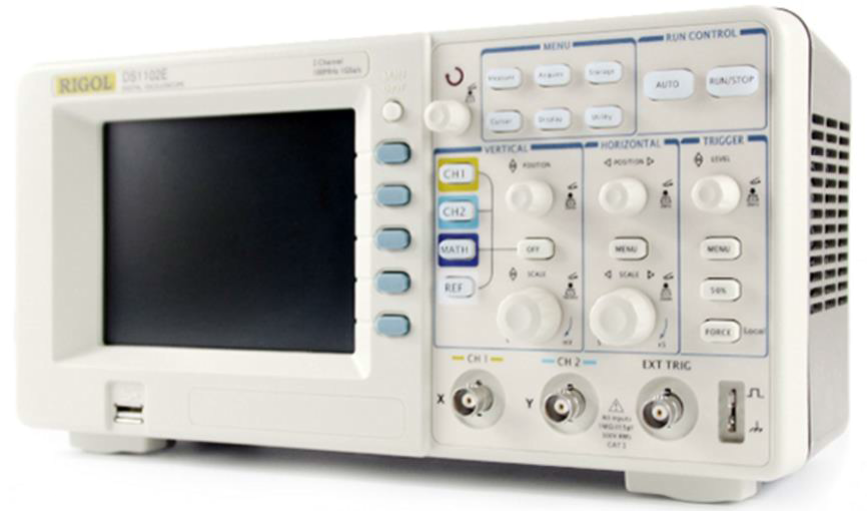
\includegraphics[width=0.9\textwidth]{数字存储示波器实物图.png}
 \end{figure}
 
  \begin{figure}[!htb]
 	\centering
 	\caption{示波器控制面板}
 	\label{示波器控制面板}
 	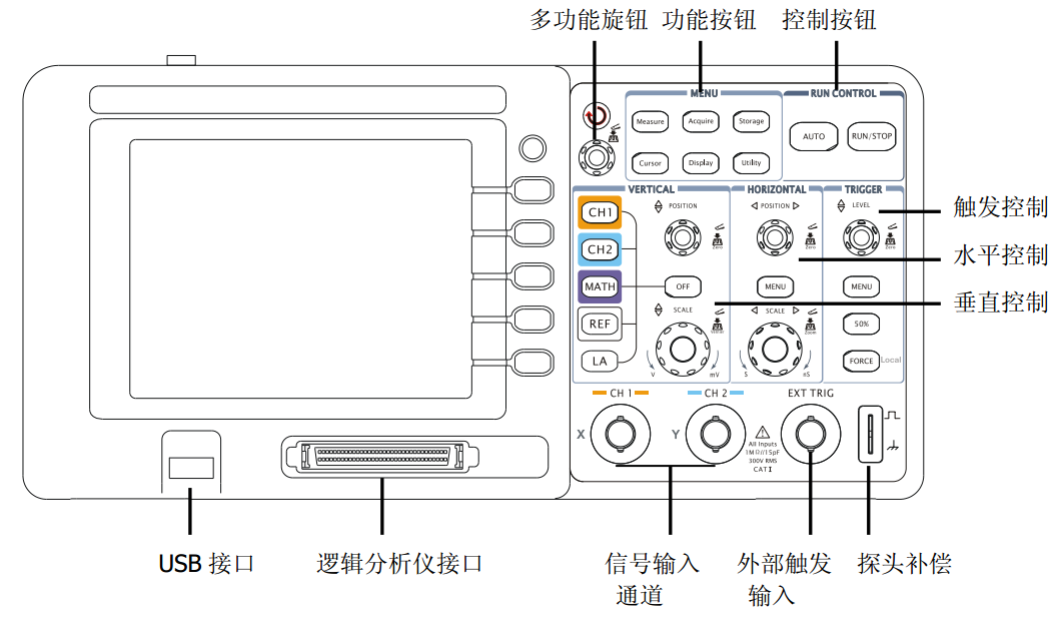
\includegraphics[width=0.9\textwidth]{示波器控制面板.png}
 \end{figure}

从上面两幅图中我们可以看出,示波器的控制面板上有各种按钮及旋钮。也就是说DSO除了能够显示波形及测量信号的各种参数之外,还包含了一系列的控制功能,比如触发控制、水平、竖直方向的控制等。这些功能是为了帮助我们获取期望的触发信号,同时方便我们去观察、分析信号波形。下面介绍几组用示波器测量信号时常用的功能键:

 \begin{enumerate}[label=(\arabic*)]
 	\item \textbf{运行控制(Run Control)}
 	\begin{enumerate}[label=\protect\ding{\numexpr171+\arabic*}]
 		\item \textbf{自动设置(AUTO)}:数字示波器一般具有自动设置的功能。根据输入的信号,可自动调整电压倍率、时基、以及触发方式使波形以最好的形态显示。
 		\item \textbf{运行/停止(RUN/STOP)}:运行时可以实时观测波形的动态变化,停止时可以静态地观察分析信号。
 	\end{enumerate}
 	\item \textbf{触发控制(Trigger)}
 	\begin{enumerate}[label=\protect\ding{\numexpr171+\arabic*}]
 		\item \textbf{触发边沿(EDGE)}:可以选择在波形的上升沿或者下降沿来触发信号的采集、存储和显示。
 		\item \textbf{触发电平(LEVEL)}:可以增大或减小触发电平,信号到达触发电平的位置时才满足触发条件。
 	\end{enumerate}
 	\item \textbf{水平控制(Horizontal)}
 	\begin{enumerate}[label=\protect\ding{\numexpr171+\arabic*}]
 		\item \textbf{位置(POSITION)}:调整信号在波形窗口的水平位置,使波形在水平方向左移或者右移。
 		\item \textbf{缩放(SCALE)}:改变水平档位,即水平方向上每格所代表的时间,单位为 s/div(秒/格)。
 	\end{enumerate}
 	\item \textbf{竖直控制(Vertical)}
 	\begin{enumerate}[label=\protect\ding{\numexpr171+\arabic*}]
 		\item \textbf{位置(POSITION)}:调整信号在波形窗口的竖直显示位置,使波形在竖直方向上移或者下移。
 		\item \textbf{缩放(SCALE)}:改变竖直档位,即竖直方向上每格所代表的电压,单位为 V/div(伏/格)。
 	\end{enumerate}
 \end{enumerate}
	
\subsection{设计任务}
我们要利用野火fpga高速AD/DA模块,在征途FPGA开发板上实现一个数字存储示波器,利用5寸RGB屏显示波形和界面。要求能够测量信号的频率和峰峰值,同时实现波形的运行控制、触发控制以及水平和竖直方向控制。

\section{设计步骤}
\subsection{硬件设计}
本项目用到了野火fpga征途pro开发板、野火高速AD/DA模块,以及5寸RGB TFT-LCD模块

首先,我们把示波器的功能实现划分为两部分,“波形的绘制”和“用户界面的绘制”。其中由于波形的实时显示对图像的刷新速率要求较高,因此适合用硬件来实现,即采用Verilog HDL来设计;而用户界面的绘制比较复杂,适合用软件来实现,即在嵌入式处理器Nios II中采用C语言来设计。

整个系统的实现方案,如下图所示:
  \begin{figure}[!htb]
	\centering
	\caption{示波器系统框图}
	\label{示波器系统框图}
	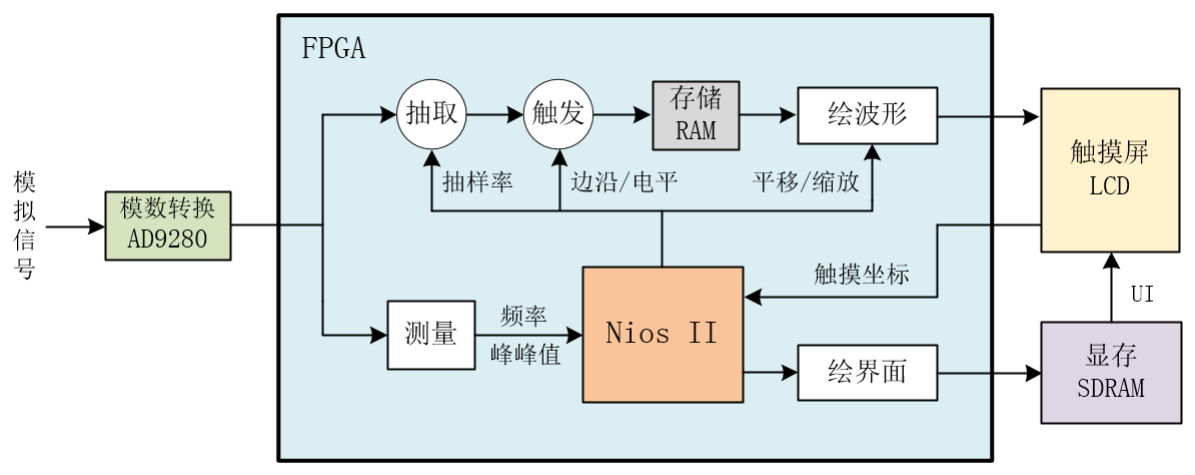
\includegraphics[width=0.9\textwidth]{示波器系统框图.png}
\end{figure}

外部的模拟信号,经过高速AD/DA模块上的模数转换器AD9280,转换成8位数字信号输入FPGA。进入FPGA后该数字信号分成两路,一路输入到测量模块,用于测量信号的频率和峰峰值;另外一路需要对数据进行抽样,抽取后的数据写到双口RAM中,在此过程中还要不停地判断触发条件,一旦满足触发条件,就记录此时的RAM地址用于绘制波形。

在整个过程中,Nios II通过Avalon-MM端口控制各个模块的工作,比如读取信号的频率和峰峰值、设置抽取过程中的抽样率、设置触发条件、以及控制波形的平移和缩放等。除此之外,Nios II还负责完成用户界面(User Interface, UI)的绘制,并根据触摸屏输入的触摸点坐标来判断用户的按键操作。

上图中SDRAM用作UI绘制过程中的显存,RGB LCD驱动模块从显存中读出UI,并与Verilog绘制的波形叠加后显示在屏幕上,从而完成示波器的显示部分。

整个系统的设计方案确定之后,我们还需要完成用户界面的设计。这里只是把期望的用
户界面用绘图工具给画出来,并不包括具体的实现。根据实验任务的要求,用户界面应该包含13个按键用来实现波形的控制,同时能够显示测量信号的参数。为了方便用户操作,还应该包含示波器当前的设置信息。最终设计出来的用户界面如下图所示: 
  \begin{figure}[!htb]
	\centering
	\caption{用户界面}
	\label{用户界面}
	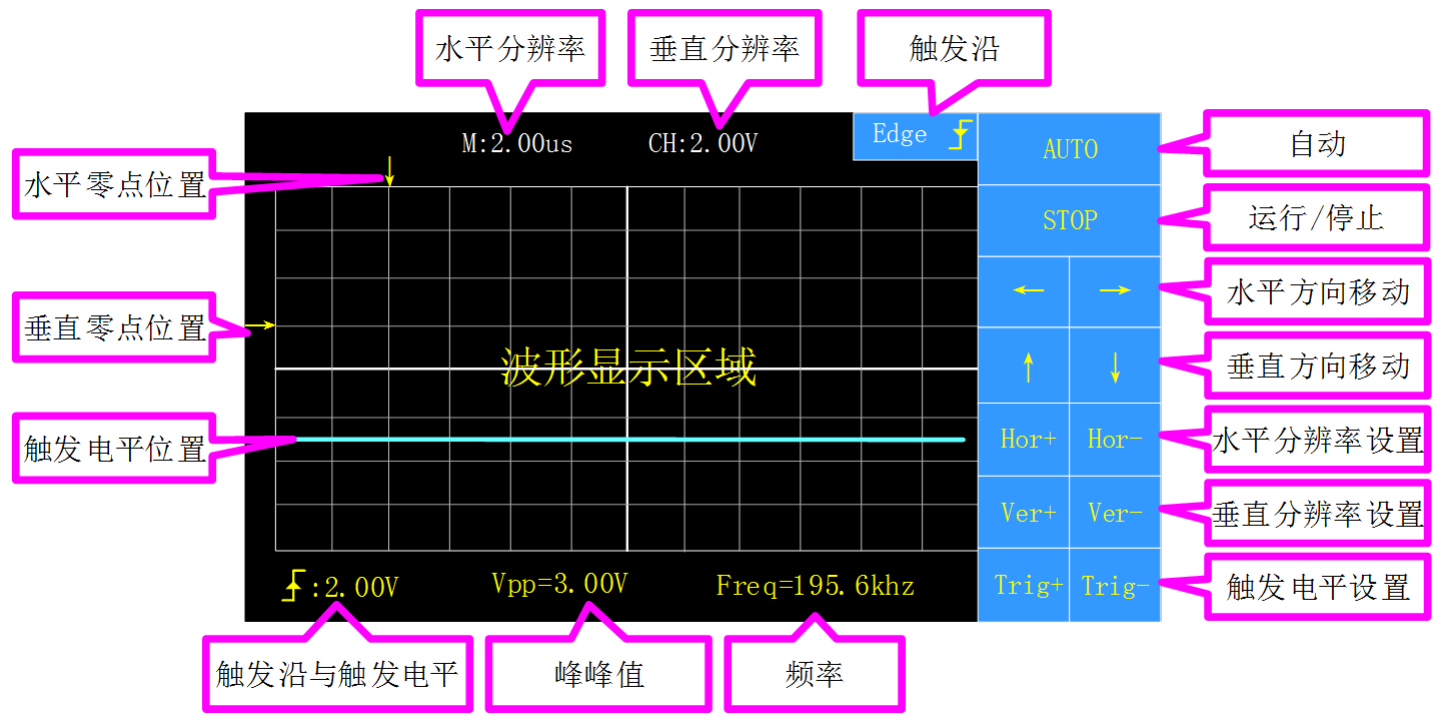
\includegraphics[width=0.9\textwidth]{用户界面.png}
\end{figure}
上面的UI设计我们将在Nios II中采用uC/GUI来实现,这部分内容会在接下来的软件设计
中讨论,我们先对照着图 \ref{示波器系统框图}来看一下底层硬件中各个模块的设计思路。
\subsubsection{测量模块}
参数测量模块param\_measure负责测量输入信号的峰峰值和频率,其模块接口定义如下图所示: 
\begin{figure}[ht]
	\begin{minipage}[t]{0.48\textwidth}
		\centering
		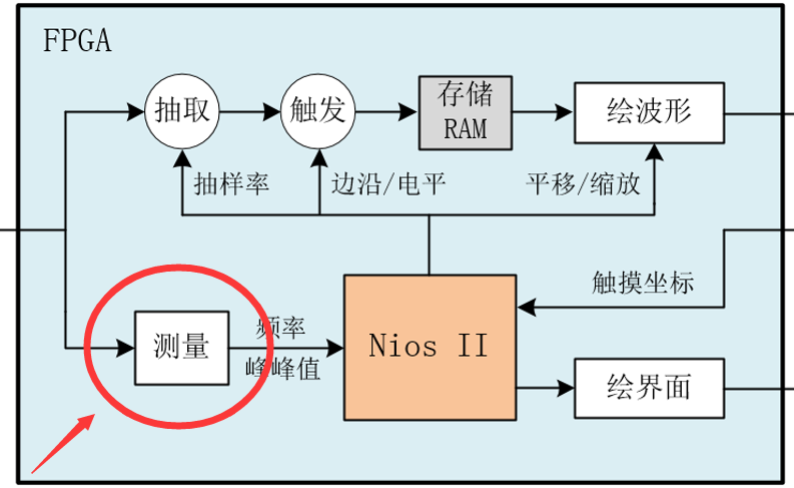
\includegraphics[width=\linewidth]{测量模块.png}
		\caption{测量模块}
		\label{fig:image1}
	\end{minipage}
	\hfill % 添加一些水平间隔
	\begin{minipage}[t]{0.48\textwidth}
		\centering
		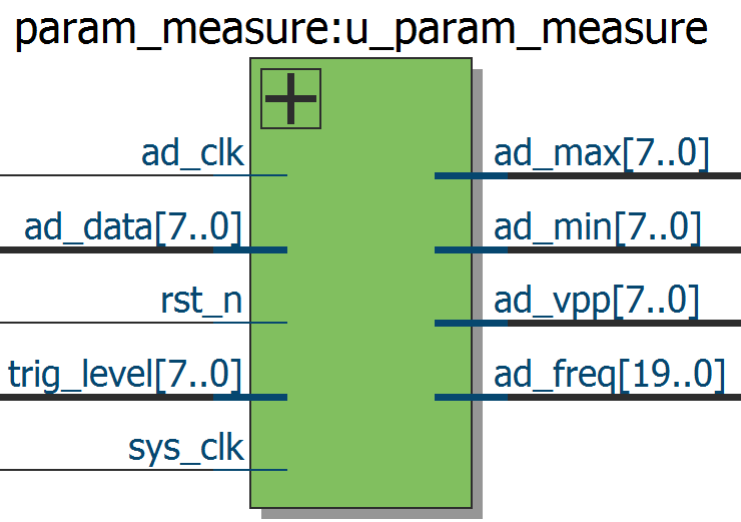
\includegraphics[width=\linewidth]{测量模块接口定义.png}
		\caption{测量模块接口定义}
		\label{fig:image2}
	\end{minipage}
\end{figure}
模块输入端除了AD采样时钟ad\_clk和采样数据ad\_data之外,还有一个信号trig\_level,这个是用户所设置的触发电平。模块输出端包括信号的最大值、最小值、峰峰值(最大值减最小值)以及信号的频率。

参数测量模块内部例化了3个子模块,如下图所示: 
  \begin{figure}[!htb]
	\centering
	\caption{参数测量模块框图}
	\label{参数测量模块框图}
	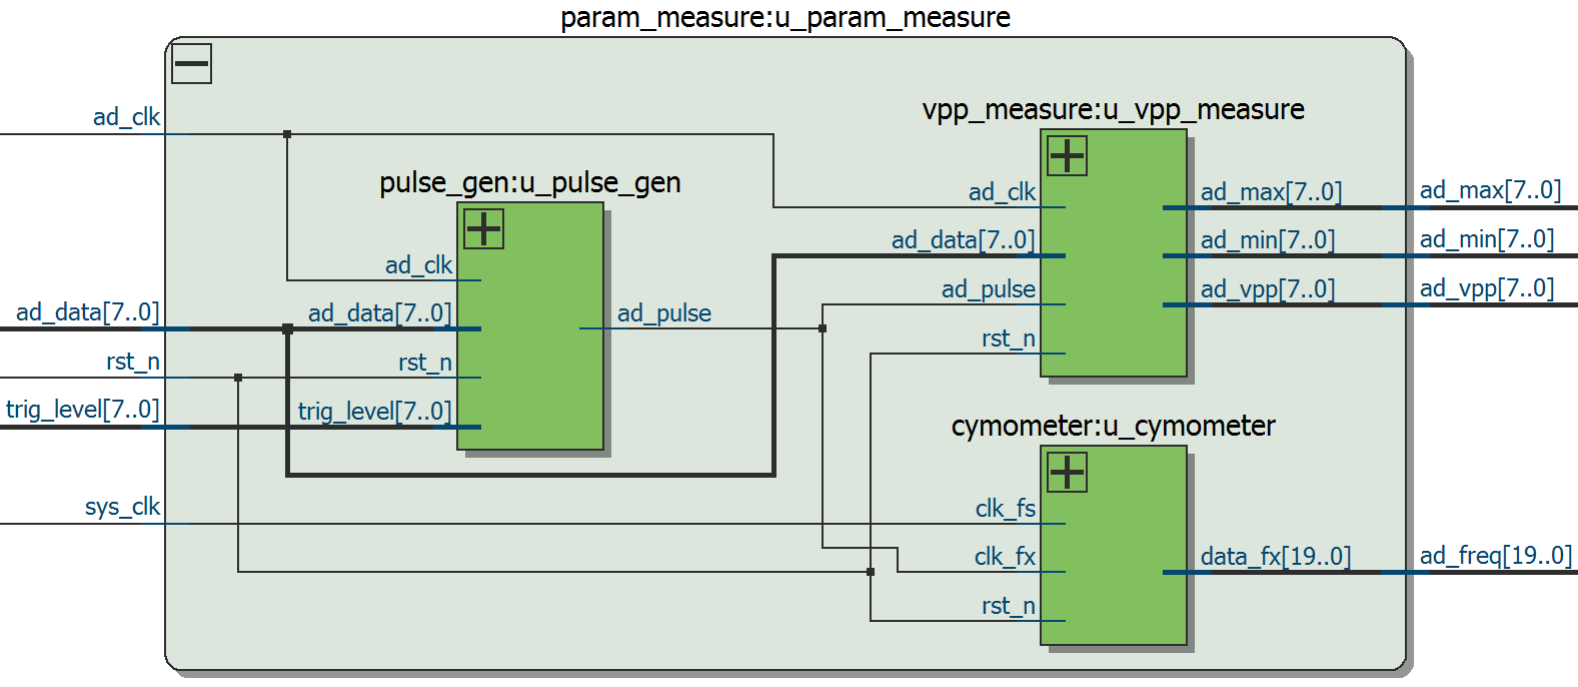
\includegraphics[width=0.9\textwidth]{参数测量模块框图.png}
\end{figure}

3个子模块中,峰峰值测量模块(vpp\_measure)和频率计模块(cymometer)分别负责测量信号的峰峰值和频率。其中,频率计模块直接调用了我们在“频率计实验”中所设计的等精度频率计;而峰峰值测量模块则通过不断地比较在一个信号周期内输入的AD采样值的大小,筛选出最大值和最小值,从而计算出信号的峰峰值。

需要注意的是,等精度频率计的输入信号是高低电平,而AD采样后得到的是8位数据ad\_data,因此我们需要根据输入的触发电平trig\_level将输入信号转换成高低电平(脉冲)。

脉冲生成模块(pulse\_gen)就是用来完成上述的过程,方法很简单,判断输入信号与触发电平的大小:当ad\_data大于trig\_level时,输出的脉冲ad\_pulse为高电平,反之为低电平。如下图所示:
  \begin{figure}[!htb]
	\centering
	\caption{脉冲生成}
	\label{脉冲生成}
	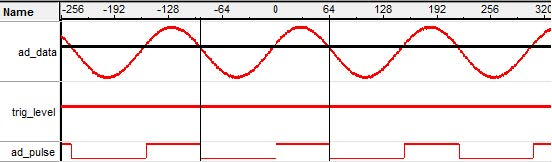
\includegraphics[width=0.9\textwidth]{脉冲生成.jpg}
\end{figure}
脉冲生成模块( pulse\_gen)就是用来完成上述的过程, 代码如下:
\begin{lstlisting}
module pulse_gen(
    input rst_n, // 系统复位,低电平有效
    input [7:0] trig_level,
    input ad_clk, // AD9280 驱动时钟
    input [7:0] ad_data, // AD 输入数据
    output ad_pulse // 输出的脉冲信号
);

parameter THR_DATA = 3;

// reg define
reg pulse;
reg pulse_delay;

// 主要代码
assign ad_pulse = pulse & pulse_delay;

// 根据触发电平,将输入的 AD 采样值转换成高低电平
always @(posedge ad_clk or negedge rst_n) begin
    if (!rst_n)
        pulse <= 1'b0;
    else begin
        if ((trig_level >= THR_DATA) && (ad_data < trig_level - THR_DATA))
            pulse <= 1'b0;
        else if (ad_data > trig_level + THR_DATA)
            pulse <= 1'b1;
    end
end

// 延时一个时钟周期,用于消除抖动
always @(posedge ad_clk or negedge rst_n) begin
    if (!rst_n)
        pulse_delay <= 1'b0;
    else
        pulse_delay <= pulse;
end

endmodule

\end{lstlisting}
峰峰值测量模块同样是利用pulse\_gen模块所输出的脉冲ad\_pulse来标识输入信号的周期,从而筛选出每个周期内的最大值和最小值。代码如下:
\begin{lstlisting}
module vpp_measure(
    input rst_n, // 复位信号
    input ad_clk, // AD 时钟
    input [7:0] ad_data, // AD 输入数据
    input ad_pulse, // 由 AD 波形得到的脉冲信号
    output reg [7:0] ad_vpp, // AD 峰峰值
    output reg [7:0] ad_max, // AD 最大值
    output reg [7:0] ad_min // AD 最小值
);

// reg define
reg vpp_flag; // 测量峰峰值标志信号
reg vpp_flag_d; // vpp_flag 延时
reg [7:0] ad_data_max; // AD 一个周期内的最大值
reg [7:0] ad_data_min; // AD 一个周期内的最小值

// wire define
wire vpp_flag_pos; // vpp_flag 上升沿标志信号
wire vpp_flag_neg; // vpp_flag 下降沿标志信号

// 边沿检测,捕获信号上升/下降沿
assign vpp_flag_pos = (~vpp_flag_d) & vpp_flag;
assign vpp_flag_neg = vpp_flag_d & (~vpp_flag);

// 利用 vpp_flag 标志一个被测时钟周期
always @(posedge ad_pulse or negedge rst_n) begin
    if (!rst_n)
        vpp_flag <= 1'b0;
    else
        vpp_flag <= ~vpp_flag;
end

// 将 vpp_flag 延时一个 AD 时钟周期
always @(posedge ad_clk or negedge rst_n) begin
    if (!rst_n)
        vpp_flag_d <= 1'b0;
    else
        vpp_flag_d <= vpp_flag;
end

// 筛选一个被测时钟周期内的最大/最小值
always @(posedge ad_clk or negedge rst_n) begin
    if (!rst_n) begin
        ad_data_max <= 8'd0;
        ad_data_min <= 8'd0;
    end else if (vpp_flag_pos) begin // 被测时钟周期开始时寄存 AD 数据
        ad_data_max <= ad_data;
        ad_data_min <= ad_data;
    end else if (vpp_flag_d) begin
        if (ad_data > ad_data_max)
            ad_data_max <= ad_data; // 计算最大值
        if (ad_data < ad_data_min)
            ad_data_min <= ad_data; // 计算最小值
    end
end

// 计算被测时钟周期内的峰峰值
always @(posedge ad_clk or negedge rst_n) begin
    if (!rst_n) begin
        ad_vpp <= 8'd0;
        ad_max <= 8'd0;
        ad_min <= 8'd0;
    end else if (vpp_flag_neg) begin
        ad_vpp <= ad_data_max - ad_data_min;
        ad_max <= ad_data_max;
        ad_min <= ad_data_min;
    end
end

endmodule

\end{lstlisting}
\subsubsection{抽取模块}
抽取模块decimator负责对输入的AD数据进行抽样,其模块接口定义如下图所示: 
\begin{figure}[ht]
	\begin{minipage}[t]{0.48\textwidth}
		\centering
		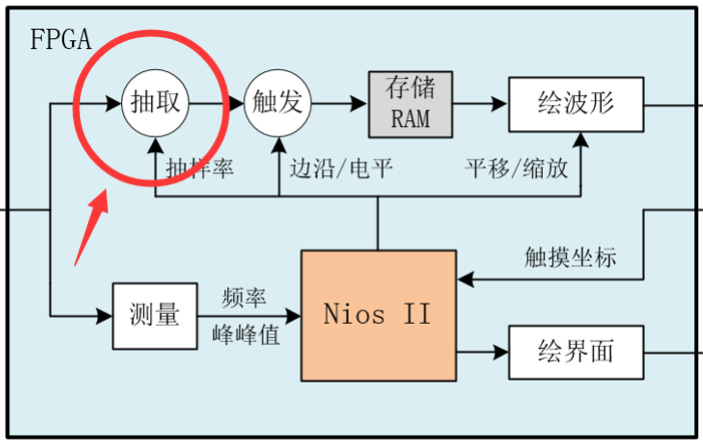
\includegraphics[width=\linewidth]{抽取模块.png}
		\caption{抽取模块}
		\label{fig:抽取模块}
	\end{minipage}
	\hfill % 添加一些水平间隔
	\begin{minipage}[t]{0.48\textwidth}
		\centering
		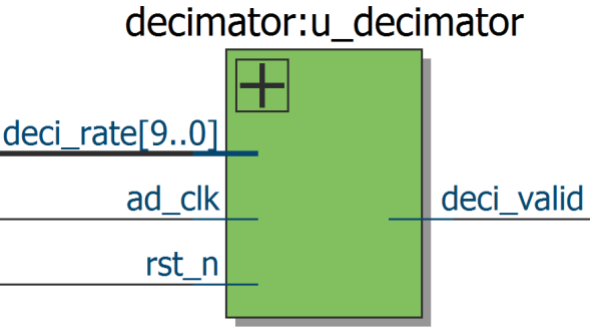
\includegraphics[width=\linewidth]{抽取模块接口定义.png}
		\caption{抽取模块接口定义}
		\label{fig:抽取模块接口定义}
	\end{minipage}
\end{figure}
抽取模块代码如下:
\begin{lstlisting}
module decimator(
    input ad_clk,
    input rst_n,
    input [9:0] deci_rate,
    output reg deci_valid
);

// reg define
reg [9:0] deci_cnt; // 抽样计数器

// 主要代码
// 抽样计数器计数
always @(posedge ad_clk or negedge rst_n) begin
    if (!rst_n)
        deci_cnt <= 10'd0;
    else if (deci_cnt == deci_rate - 1)
        deci_cnt <= 10'd0;
    else
        deci_cnt <= deci_cnt + 1'b1;
end

// 输出抽样有效信号
always @(posedge ad_clk or negedge rst_n) begin
    if (!rst_n)
        deci_valid <= 1'b0;
    else if (deci_cnt == deci_rate - 1)
        deci_valid <= 1'b1;
    else
        deci_valid <= 1'b0;
end

endmodule

\end{lstlisting}
抽取模块的接口比较简单,根据输入端的抽样率deci\_rate,输出抽取有效信号deci\_valid。实际上它的工作原理也很简单,我们只需要定义一个计数器,每次计数到所设置的抽样率就输出一个抽取有效信号,然后从0开始重新计数。比如说抽样率为10,那么每隔10个时钟周期就输出一个时钟周期的有效信号,也就是说AD采集到的连续十个数据中只有一个是有效的。

那么我们抽样的目的是什么呢?因为AD的采样率比较高,本次里输出的AD时钟ad\_clk为30MHz。假设输入的模拟信号是频率为1MHz的正弦波,那么每个周期的信号AD可以采到30个数据。我们屏幕上用来显示波形的区域在水平方向上有300个像素点,那么就可以显示10个周期的信号波形,每个周期由30个点组成。

但是如果输入的模拟信号频率为1KHz,那么每个周期AD可以采到30\_000个数据(30MHz/1KHz)。如果AD得到的每个数据都用来绘制波形的话,那么满屏就只能够显示该信号0.01个周期的波形,也就是一个周期正弦波的百分之一。此时我们在屏幕上看到的波形根本看不出来是个正弦波,可能就是一小段斜线。

在这个时候我们就需要对AD得到的数据进行抽样,等间距地每1000个点取一个用于绘制波形,那么每个信号周期可以抽样到30个点。这样就可以在屏幕上看到10个周期的正弦波,此时的抽样率就是1000。如果此时抽样率是100,那么一个信号周期里刚好可以抽取300个数据用于绘制波形,刚好铺满整个波形区域。

在抽样率从1000减小到100的过程中,屏幕上显示的波形从10个周期变成了1个周期,相当于波形在水平方向上进行了放大,这样就方便我们观察波形的细节。同理,如果我们需要在水平方向上缩小波形的话,就增加抽样率,这样就可以同时观察多个周期的波形。

\subsubsection{触发和存储模块}
触发模块负责检测信号何时满足触发条件,而存储模块则将抽取之后的AD数据存到双口RAM中。由于这两个模块关联比较紧密,因此在本次设计中将触发模块并入存储模块data\_store中,其接口定义如下所示:
\begin{figure}[ht]
	\begin{minipage}[t]{0.48\textwidth}
		\centering
		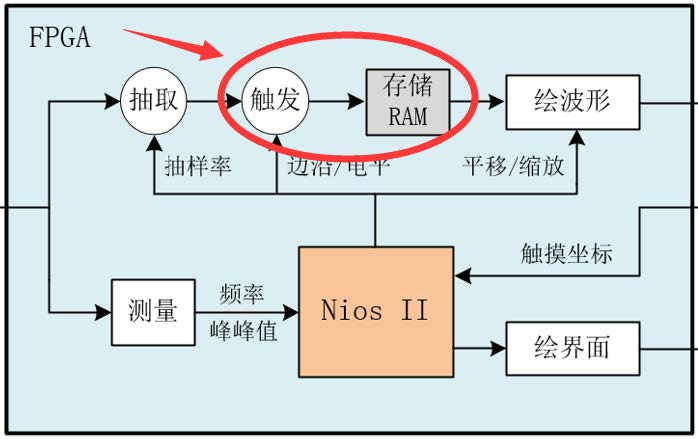
\includegraphics[width=\linewidth]{存储模块.jpg}
		\caption{存储模块}
		\label{fig:存储模块}
	\end{minipage}
	\hfill % 添加一些水平间隔
	\begin{minipage}[t]{0.48\textwidth}
		\centering
		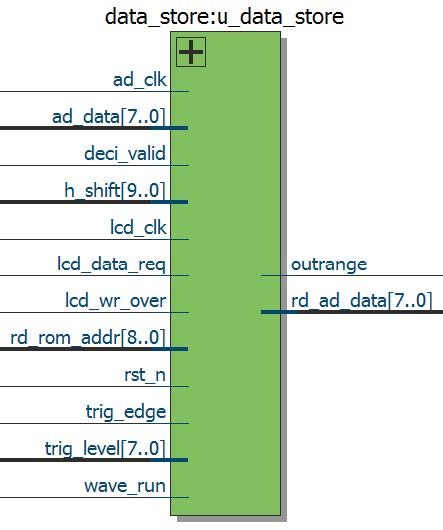
\includegraphics[width=\linewidth]{存储模块接口定义.jpg}
		\caption{存储模块接口定义}
		\label{fig:存储模块接口定义}
	\end{minipage}
\end{figure}
数字存储示波器的一个优点就是我们可以同时观察到触发条件发生前后的信号波形。触发条件包括触发电平(trig\_level)和触发沿(trig\_edge),可以看到这两个条件都是存储模块(data\_store)的输入信号。如果设置的是上升沿触发,那么在抽样后的AD数据到达触发电平时,还要判断前一个数据是否小于触发电平。如果前一个数据小于触发电平,同时当前数据大于或等于触发电平,那么就满足触发条件。同样,如果是下降沿触发,就要判断前一个数据是否大于触发电平。

数字存储示波器为了能够在停止运行(STOP)的时候重现波形,需要将AD得到的数据存储起来,然后再用于绘制波形。在这里我们例化一个双口RAM用于存储AD数据,存储深度为300,即波形显示区域的水平方向的分辨率。当抽样有效信号deci\_valid拉高时,将抽样后的数据写入RAM中,写入的地址从0开始依次累加,累加到299的时候地址归零,如此周而复始。

在这里我们需要注意的是,为了能够观察触发时刻前后的信号波形,我们需要记录触发点数据写入RAM的地址。在达到触发条件后,我们继续存储150个数据,然后等待波形绘制结束。这样的话,在触发点前后波形数据各占一半。为了使触发点处于波形显示区域的中间位置,我们要根据记录的触发点数据的RAM地址,计算出当前所绘制波形的第一个点的RAM地址,然后向后依次读出300个点,在波形显示区域里从左向右依次绘制波形。

在前面我们讲过改变抽样率的大小可以完成波形在水平方向上的缩放,那么水平方向上的平移怎么实现呢?数据存储模块的输入端有一个h\_shift信号,它指示波形在水平方向上平移的距离。我们根据h\_shift的值,改变读RAM的地址就可以了。比如波形左移的话,读RAM的地址应该加上h\_shift,相当于把右侧的波形数据显示在了当前位置;同理,波形右移的话,读RAM的地址应该减去h\_shift。

data\_store 模块代码如下:
\begin{lstlisting}
module data_store(
    input rst_n, // 复位信号
    input [7:0] trig_level, // 触发电平
    input trig_edge, // 触发边沿
    input wave_run, // 波形采集启动/停止
    input [9:0] h_shift, // 波形水平偏移量
    input ad_clk, // AD 时钟
    input [7:0] ad_data, // AD 输入数据
    input deci_valid, // 抽样有效信号
    input lcd_clk,
    input lcd_wr_over,
    input wave_data_req,
    input [8:0] wave_rd_addr,
    output [7:0] wave_rd_data,
    output reg outrange // 水平偏移超出范围
);

// reg define
reg [8:0] wr_addr; // RAM 写地址
reg ram_aclr; // RAM 清除
reg trig_flag; // 触发标志
reg trig_en; // 触发使能
reg [8:0] trig_addr; // 触发地址
reg [7:0] pre_data;
reg [7:0] pre_data1;
reg [7:0] pre_data2;
reg [8:0] data_cnt;

// wire define
wire wr_en; // RAM 写使能
wire [9:0] rd_addr; // RAM 地址
wire [9:0] rel_addr; // 相对触发地址
wire [9:0] shift_addr; // 偏移后的地址
wire trig_pulse; // 满足触发条件时产生脉冲
wire [7:0] rd_ram_data;

// 主要代码
assign wr_en = deci_valid && (data_cnt <= 299) && wave_run;

// 计算波形水平偏移后的 RAM 数据地址
assign shift_addr = h_shift[9] ? (wave_rd_addr - h_shift[8:0]) : (wave_rd_addr + h_shift[8:0]);

// 根据触发地址,计算像素横坐标所映射的 RAM 地址
assign rel_addr = trig_addr + shift_addr;
assign rd_addr = (rel_addr < 150) ? (rel_addr + 150) :
                 (rel_addr > 449) ? (rel_addr - 450) :
                 (rel_addr - 150);

// 满足触发条件时输出脉冲信号
assign trig_pulse = trig_edge ?
                    ((pre_data2 < trig_level) && (pre_data1 < trig_level) && (pre_data >= trig_level) && (ad_data > trig_level)) :
                    ((pre_data2 > trig_level) && (pre_data1 > trig_level) && (pre_data <= trig_level) && (ad_data < trig_level));

// 读出的数据为 255 时超出波形显示范围
assign wave_rd_data = outrange ? 8'd255 : (8'd255 - rd_ram_data);

\end{lstlisting}
程序中第 45 行代码为 RAM 写使能进行赋值, 可以发现,只要输入的数据有效( deci\_valid=1)、 data\_cnt的值小于等于 299,且示波器处于运行状态,则持续向 RAM 中写入数据。

程序中第 48 行和 49 行代码,根据输入的波形水平像素偏移量,计算偏移后的 RAM 地址( shift\_addr),直接在 wave\_rd\_addr 的基础上,根据左移或者右移,对 h\_shift 的低 9 位进行加减即可。
程序中第 52行代码,是根据满足触发条件时的触发地址和偏移后的地址,计算实际上的 RAM 地址。

程序中第 53 行至 55 行代码,为实际连接到 RAM 端口上的读地址( rd\_addr)进行赋值, 这里根据 rel\_addr值的大小,来计算 rd\_addr。 我们知道,在满足触发条件后,会继续向 RAM 中写入 150 个数据,所以在从RAM 中读取数据时,第一个要显示的点,应该是最早一次写入 RAM 的数据;而最后一次从 RAM 中读到的数据,应该是最后一次向 RAM 中写入的数据, 该行代码就是实现此功能。

程序中第 58 行至 62 行代码根据输入的触发类型( trig\_edge) ,来产生满足触发脉冲信号( trig\_pulse),当满足条件时, trig\_edge 为高电平,否则为低电平。

程序中第 65 行代码, 为 wave\_rd\_data 信号进行赋值。当 outrange 为高电平( 超出显示边界) ,固定赋值为 255, 否则等于 255-rd\_ram\_data。 由于输入模拟电压值越高, rd\_ram\_data 的值越大, 在 RGB LCD 屏上显示的位置应越接近于上侧, 而 RGB LCD 屏 Y 方向像素点从上往下扫描,且 Y 方向的计数器从上往下依次累加,因此输出给 LCD 顶层模块的wave\_rd\_data,进行了数值处理,即用 255 减去 rd\_ram\_data。
\begin{lstlisting}[firstnumber=67]
// 判断水平偏移后地址范围
always @(posedge lcd_clk or negedge rst_n) begin
    if (!rst_n)
        outrange <= 1'b0;
    else if (h_shift[9] && (wave_rd_addr < h_shift[8:0])) // 右移时判断左边界
        outrange <= 1'b1;
    else if ((~h_shift[9]) && (wave_rd_addr + h_shift[8:0] > 299)) // 左移时判断右边界
        outrange <= 1'b1;
    else
        outrange <= 1'b0;
end

// 写 RAM 地址累加
always @(posedge ad_clk or negedge rst_n) begin
    if (!rst_n)
        wr_addr <= 9'd0;
    else if (deci_valid) begin
        if (wr_addr < 9'd299)
            wr_addr <= wr_addr + 1'b1;
        else
            wr_addr <= 9'd0;
    end
end

// 触发使能
always @(posedge ad_clk or negedge rst_n) begin
    if (!rst_n) begin
        data_cnt <= 9'd0;
        trig_en <= 1'b0;
    end else begin
        if (deci_valid) begin
            if (data_cnt < 149) begin // 触发前至少接收 150 个数据
                data_cnt <= data_cnt + 1'b1;
                trig_en <= 1'b0;
            end else begin
                trig_en <= 1'b1; // 打开触发使能
                if (trig_flag) begin // 检测到触发信号
                    trig_en <= 1'b0;
                    if (data_cnt < 300) // 继续接收 150 个数据
                        data_cnt <= data_cnt + 1'b1;
                end
            end
        end
        // 波形绘制完成后重新计数
        if ((data_cnt == 300) && lcd_wr_over & wave_run)
            data_cnt <= 9'd0;
    end
end

\end{lstlisting}
程序中第 68 行至 79 行代码根据输入的水平偏移量,来判断波形是否移出左右边界,当移出边界后,拉高 outrange 信号,此时 LCD顶层模块会根据该信号的值,来判断当前 LCD 像素点显示 UI 界面还是波形数据。

程序中第 82 行至 91 行代码根据抽样有效信号( deci\_valid),循环对写 RAM 地址进行累加,地址范围是 0~299,共 300 个存储地址。

程序中第 94 行至 119 行代码对触发使能信号和数据计数器进行赋值。 在开始查找触发点之前,先至少接收 150 个数据,满足条件后,拉高 trig\_en信号,此时开始检测满足条件的触发点,并且 data\_cnt 停止累加(但与此同时,新采样的 AD 数据会继续写入 RAM 中,以保证 AD 数据是连续的)。当检测到满足触发条件后,拉低 trig\_en 信号,继续接收 150 个数据。
\begin{lstlisting}[firstnumber=121]
// 寄存 AD 数据,用于判断触发条件
always @(posedge ad_clk or negedge rst_n) begin
    if (!rst_n) begin
        pre_data <= 8'd0;
        pre_data1 <= 8'd0;
        pre_data2 <= 8'd0;
    end else if (deci_valid) begin
        pre_data <= ad_data;
        pre_data1 <= pre_data;
        pre_data2 <= pre_data1;
    end
end

// 触发检测
always @(posedge ad_clk or negedge rst_n) begin
    if (!rst_n) begin
        trig_addr <= 9'd0;
        trig_flag <= 1'b0;
    end else begin
        if (deci_valid && trig_en && trig_pulse) begin
            trig_flag <= 1'b1;
            trig_addr <= wr_addr + 2;
        end
        if (trig_flag && (data_cnt == 300) && lcd_wr_over && wave_run)
            trig_flag <= 1'b0;
    end
end

// 例化双口 RAM
ram_2port u_ram_2port (
    .wrclock (ad_clk),
    .wraddress (wr_addr),
    .data (ad_data),
    .wren (wr_en),
    .rdclock (lcd_clk),
    .rd_aclr (1'b0),
    .rdaddress (rd_addr),
    .rden (wave_data_req),
    .q (rd_ram_data)
);

endmodule

\end{lstlisting}
程序中第 122 行代码至 150 行代码根据输入的触发条件,检测满足触发条件的位置,检测的方法也比较简单。 如果设置的是上升沿触发, 那么在抽样后的 AD 数据到达触发电平时, 还要判断前一个数据是否小于触发电平。 如果前一个数据小于触发电平,同时当前数据大于或等于触发电平,那么就满足触发条件。

同样,如果是下降沿触发,就要判断前一个数据是否大于触发电平。程序中最后例化的 ram\_2port 是 Quartus 软件自带的 RAM IP 核, 用来存储 AD 数据。
\subsubsection{绘波形模块}
波形绘制模块负责根据从存储模块读出的AD数据来绘制波形,其接口定义如下所示:
\begin{figure}[ht]
	\begin{minipage}[t]{0.48\textwidth}
		\centering
		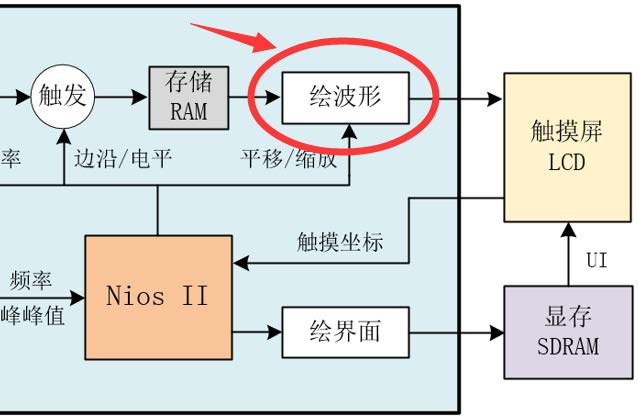
\includegraphics[width=\linewidth]{绘波形模块.jpg}
		\caption{绘波形模块}
		\label{fig:绘波形模块}
	\end{minipage}
	\hfill % 添加一些水平间隔
	\begin{minipage}[t]{0.48\textwidth}
		\centering
		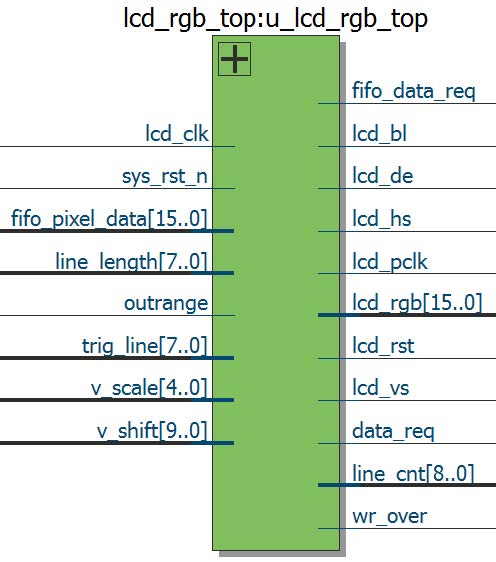
\includegraphics[width=\linewidth]{绘波形模块接口定义.jpg}
		\caption{绘波形模块接口定义}
		\label{fig:绘波形模块接口定义}
	\end{minipage}
\end{figure}

在波形绘制模块的输入端有两个信号v\_scale和v\_shift,这两个信号控制着显示波形在竖直方向上的缩放和平移。这个实现起来比较简单,我们只需要根据缩放比例(v\_scale)将从RAM中读出的AD数据进行乘、除运算,然后根据竖直方向上的平移距离(v\_shift)将运算后的数据进行加、减运算即可。

波形绘制模块例化了两个子模块,如图 \ref{波形绘制模块框图}所示。其中LCD驱动模块(lcd\_driver)模块负责完成5寸RGB LCD的驱动,同时会输出当前像素点的坐标。而LCD显示模块(lcd\_display)则根据驱动模块输出的像素点坐标来控制数据请求信号(data\_req)。数据请求信号会作为RAM的读使能信号,从RAM中读出AD数据。最后显示模块根据读出的数据绘制波形,绘制波形最简单的方法就是,判断当前像素点的纵坐标是否等于读出的AD数据(line\_length),如果等于的话就把当前像素点赋值为白色(波形颜色),不等于的话就赋值为黑色(背景色)。这种方法画出来的波形是由一个个独立的点组成的虚线,我们还要在此基础上用直线把这些点连接起来。除此之外,我们还要考虑到波形的缩放和平移等其他的因素。
  \begin{figure}[!htb]
	\centering
	\caption{波形绘制模块框图}
	\label{波形绘制模块框图}
	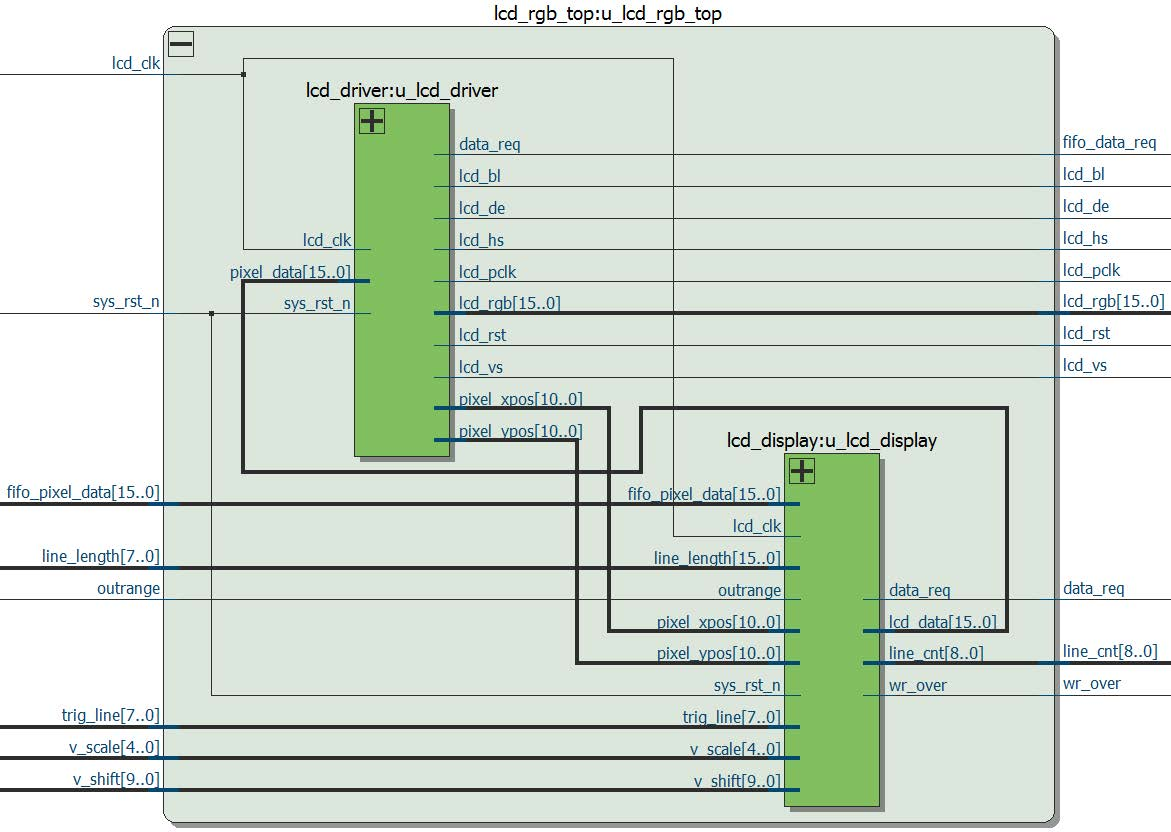
\includegraphics[width=0.9\textwidth]{波形绘制模块框图.jpg}
\end{figure}

需要注意的是,我们在这个模块中还完成了把波形和UI界面集成到一起的功能。在模块的输出端口还有一个fifo\_data\_req信号,这个信号会从显存SDRAM中请求数据,它请求的数据(fifo\_pixel\_data)就是我们所绘制的UI界面的各像素点颜色值。

我们前面在绘制波形的时候,会把波形所在的像素点赋值为白色,而背景区域赋值为黑色。现在为了把波形和UI界面叠加起来,就要把除了波形所在的像素点之外的其他区域(包括波形的黑色背景),赋值为从显存中读出的UI界面像素点颜色值(fifo\_pixel\_data)。
\begin{lstlisting}
module lcd_rgb_top(
    input clk_25m,
    input clk_12_5m,
    input rst_n, // 复位
    // RGB LCD 接口
    output lcd_de, // LCD 数据使能信号
    output lcd_hs, // LCD 行同步信号
    output lcd_vs, // LCD 场同步信号
    output lcd_clk, // LCD 像素时钟
    inout [15:0] lcd_rgb, // LCD RGB565 颜色数据
    output lcd_rst,
    output lcd_bl,
    input [9:0] v_shift, // 波形竖直偏移量
    input [4:0] v_scale, // 波形竖直缩放比例
    input [7:0] trig_line, // 触发电平
    input outrange,
    input [15:0] ui_pixel_data, // UI 像素数据
    input [7:0] wave_data,
    output ui_data_req, // UI 数据请求信号
    output [8:0] wave_addr,
    output wave_data_req, // 请求波形数据
    output wr_over,
    output [15:0] lcd_id // LCD 屏 ID
);

// 除 480*272 屏幕之外,填充黑色
parameter BACK_COLOR = 16'h0000;

wire lcd_pclk; // LCD 像素时钟
wire [10:0] pixel_xpos; // 当前像素点横坐标
wire [10:0] pixel_ypos; // 当前像素点纵坐标
wire [15:0] lcd_rgb_o; // 输出的像素数据
wire [15:0] lcd_rgb_i; // 输入的像素数据
wire [15:0] pixel_data; // 像素数据
wire data_req;
wire [15:0] display_pixel_data;
wire [8:0] clip_pixel_xpos; // 裁剪后的像素点横坐标
wire [8:0] clip_pixel_ypos; // 裁剪后的像素点纵坐标

reg ui_data_req_d0;

// 像素数据方向切换
assign lcd_rgb = lcd_de ? lcd_rgb_o : {16{1'bz}};
assign lcd_rgb_i = lcd_rgb;
// 选择输出 UI 和波形像素点或者填充的像素(填充黑色)
assign pixel_data = ui_data_req_d0 ? display_pixel_data : BACK_COLOR;

// 对 ui_data_req 信号打一拍
always @(posedge lcd_pclk or negedge rst_n) begin
    if (!rst_n) begin
        ui_data_req_d0 <= 1'b0;
    end else begin
        ui_data_req_d0 <= ui_data_req;
    end
end

endmodule

\end{lstlisting}
\subsubsection{Avalon-MM接口模块}
到这里我们示波器方案中有关参数测量及波形绘制的功能模块基本上就介绍完了,但是实际上还有一个模块是没有画出来的,就是avalmm\_interface模块。

前面我们介绍的模块它们都是由Nios II控制的,Nios II会向这些模块传递相应的控制参数,比如说触发电平、抽样率、波形的缩放比例等。而avalmm\_interface模块就是Nios II处理器与这些模块之间的接口,Nios II与avalmm\_interface模块按照Avalon-MM总线协议通信,其中Nios II作为主端口(Master),而avalmm\_interface模块实现了从端口(Slave)的功能。在avalmm\_interface模块中定义了一组寄存器,每个寄存器有对应的地址,Nios II可以根据地址将控制参数按照Avalon-MM总线协议写入相应的寄存器中,然后该模块会将这些控制参数传递到相应的各个功能模块。

avalmm\_interface模块的接口定义如下图所示:
  \begin{figure}[!htb]
	\centering
	\caption{Avalon-MM 接口模块}
	\label{Avalon-MM 接口模块}
	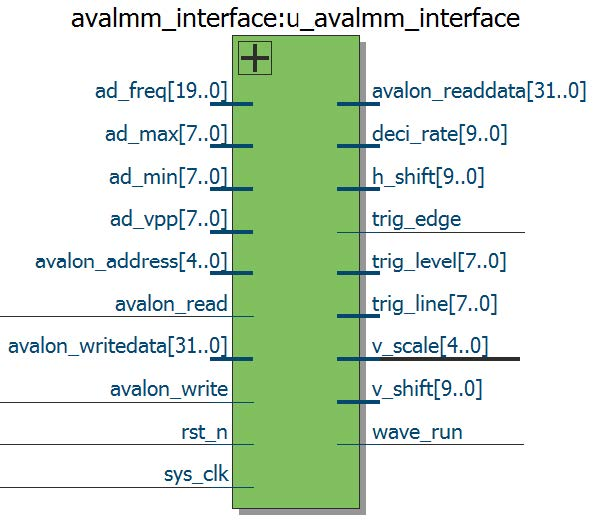
\includegraphics[width=0.5\textwidth]{Avalon-MM 接口模块.jpg}
\end{figure}
Avalon-MM 接口配置模块实现对上表中的协议进行解析, 具体代码如下:
\begin{lstlisting}
module avalmm_interface(
    input clk,
    input rst_n,
    input avalon_write, // 写指令
    input avalon_read, // 读指令
    input [31:0] avalon_writedata, // 写数据
    output [31:0] avalon_readdata, // 读数据
    input [4:0] avalon_address, // 地址线
    input [19:0] ad_freq, // AD 脉冲信号的频率
    input [7:0] ad_vpp, // AD 输入信号峰峰值
    input [7:0] ad_max, // AD 输入信号最大值
    input [7:0] ad_min, // AD 输入信号最小值
    output reg [9:0] deci_rate, // 抽样率
    output reg [7:0] trig_level, // 触发电平
    output reg [7:0] trig_line, // 触发线位置
    output reg trig_edge, // 触发边沿 0:下降沿 1:上升沿
    output reg wave_run, // 波形采集运行
    output reg [9:0] h_shift, // 波形水平偏移量
    output reg [9:0] v_shift, // 波形竖直偏移量
    output reg [4:0] v_scale // 波形竖直缩放比例
);

// reg define
reg [31:0] readdata_reg; // 读数据寄存器

// 主要代码
assign avalon_readdata = readdata_reg;

// avalon-mm 读端口
always @(posedge clk or negedge rst_n) begin
    if (!rst_n)
        readdata_reg <= 32'd0;
    else if (avalon_read) begin
        case (avalon_address)
            5'd0: readdata_reg <= {12'd0, ad_freq};
            5'd1: readdata_reg <= {8'd0, ad_vpp, ad_max, ad_min};
            default: readdata_reg <= 32'd0;
        endcase
    end
end

// avalon-mm 写端口
always @(posedge clk or negedge rst_n) begin
    if (!rst_n) begin
        deci_rate <= 10'd2;
        trig_level <= 8'd128;
        trig_line <= 8'd148;
        trig_edge <= 1'b0;
        wave_run <= 1'b1;
        h_shift <= 10'd0;
        v_shift <= 10'd0;
        v_scale <= 5'd0;
    end else if (avalon_write) begin
        case (avalon_address)
            5'd2: deci_rate <= avalon_writedata[9:0];
            5'd3: begin
                trig_level <= avalon_writedata[7:0];
                trig_line <= avalon_writedata[15:8];
            end
            5'd4: trig_edge <= avalon_writedata[0];
            5'd5: wave_run <= avalon_writedata[0];
            5'd6: h_shift <= avalon_writedata[9:0];
            5'd7: v_shift <= avalon_writedata[9:0];
            5'd8: v_scale <= avalon_writedata[4:0];
        endcase
    end
end

endmodule

\end{lstlisting}

在介绍完各功能模块后,接下来我们在软件设计部分介绍一下如何实现UI界面的绘制,以及如何利用触摸屏来实现与用户的交互。
\subsection{软件设计}
	示波器的UI界面比较复杂,包括示波器的各个功能按键、波形的频率与峰峰值、水平零点位置与垂直零点位置等。为了提高UI界面的开发效率,UI界面的绘制我们将在Nios II中采用uC/GUI来实现,这样将会大大提高UI界面的开发效率以及降低UI界面绘制的复杂度。
	
	Nios II除了负责完成用户界面的绘制外,还根据触摸屏输入的触摸点坐标来判断用户的按键操作,根据用户的按键操作给硬件的各个模块发送参数,从而控制波形的显示。触摸驱动可以在Nios II中通过C语言来编写,当然也可以在硬件中通过Verilog语言来编写。。本次实验触摸屏的驱动是在硬件中使用Verilog语言实现,Nios II通过Avalon-MM端口来获取触摸驱动模块输出的触摸点的坐标。
	
\subsubsection{触摸屏驱动模块}
事实上,触摸屏驱动模块是在硬件设计中实现的,只不过这个模块的数据接口并没有直接和其它模块做交互,而是通过Avalon-MM接口来向Nios II传输坐标值。触摸屏驱动模块完成对触摸屏按键的检测与触摸点坐标的获取,其模块接口定义如下图所示:
  \begin{figure}[!htb]
	\centering
	\caption{触摸屏驱动模块}
	\label{触摸屏驱动模块}
	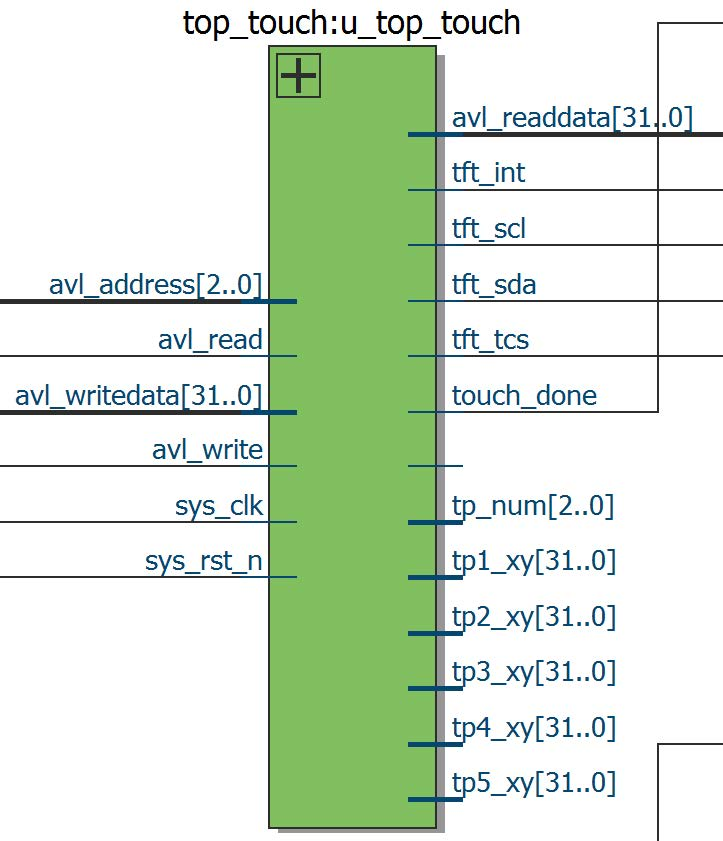
\includegraphics[width=0.5\textwidth]{触摸屏驱动模块.jpg}
\end{figure}
需要说明的是,触摸屏驱动模块只针对5寸RGB LCD屏的触摸驱动,其触摸芯片为GT9147。触摸屏驱动模块通过IIC接口检测到屏幕被按下后,会拉高touch\_done信号,并输出触摸点的个数(tp\_num)以及触摸点的坐标(tp1\_xy~tp5\_xy),不过触摸点的个数以及触摸点的坐标在本次实验并没有用到,而是通过Avalon-MM接口来向Nios II传输坐标值,这样将会大大减少Nios II和触摸屏驱动模块之间端口连接的数量

摸屏驱动模块例化了两个子模块,如图 \ref{触摸屏模块框图}所示。其中GT9147配置模块(gt9147\_cfg)用于初始化触摸屏,即通过IIC接口对GT9147进行配置,并在配置完成后拉高配置完成信号(cfg\_done)。而GT9147驱动模块(gt9147\_ctrl)负责控制触摸屏驱动的整个流程,包括控制触摸屏初始化的开始、检测触摸屏是否被按下以及读取触摸点的坐标,同时GT9147驱动模块也实现了Avalon-MM接口从端口(Slave)的功能。

  \begin{figure}[!htb]
	\centering
	\caption{触摸屏模块框图}
	\label{触摸屏模块框图}
	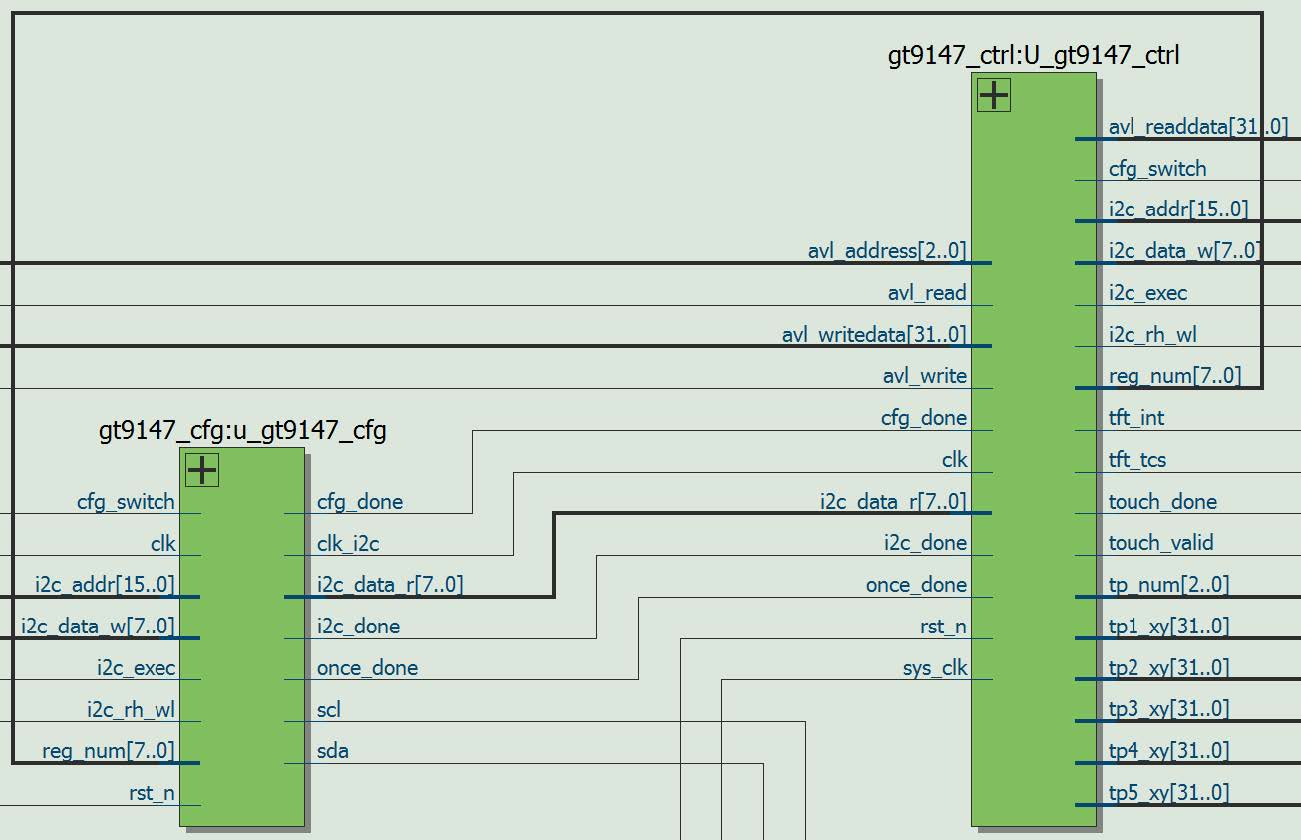
\includegraphics[width=0.5\textwidth]{触摸屏模块框图.jpg}
\end{figure}

GT9147配置模块例化了以下三个模块,分别是信号切换模块(signal\_switch)、IIC驱动模块(i2c\_dri\_m)和i2c参数配置模块(i2c\_reg\_cfg),如图 \ref{GT9147配置模块框图}所示。
  \begin{figure}[!htb]
	\centering
	\caption{GT9147配置模块框图}
	\label{GT9147配置模块框图}
	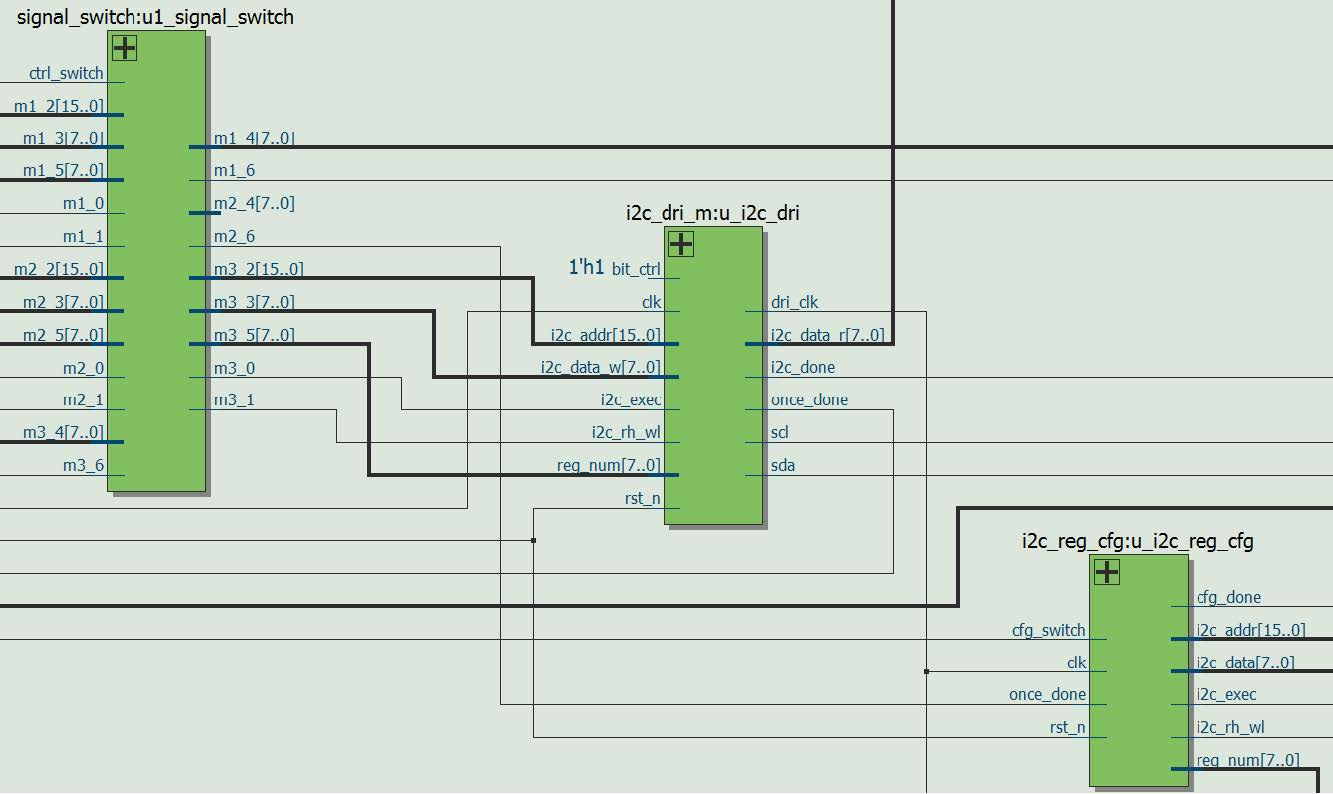
\includegraphics[width=0.5\textwidth]{GT9147配置模块框图.jpg}
\end{figure}


IIC参数配置模块寄存了触摸屏初始化参数,共需要配置186个寄存器。当输入的配置切换信号(cfg\_switch)为高电平时,开始初始化触摸屏,并在初始化完成后拉高cfg\_done信号。

由于GT9147驱动模块的读写操作和IIC参数配置模块的初始化操作都会用到IIC接口,因此这两个模块输出的端口信号需要先做一个选择,再连接到IIC的驱动模块中,信号选择的功能是由信号切换模块实现的。这个模块实现的方法也比较简单,根据输入的cfg\_switch信号的高低电平进行选择。当cfg\_switch为高电平时,将IIC参数配置模块的IIC操作端口信号连接至IIC驱动模块;当cfg\_switch为低电平时,将GT9147驱动模块的IIC操作端口信号连接至IIC驱动模块。

\subsubsection{SDRAM桥控制模块}
Nios II采用uC/GUI绘制UI界面,将像素数据写入SDRAM中,并最终显示在 RGB LCD屏上。这就要求SDRAM读出数据的速度比较快,因此我们使用具有突发读写能力的Avalon-MM Pipeline Bridge IP核来和SDRAM进行数据通信。SDRAM桥控制模块从SDRAM中读出数据,将其缓存至FIFO中,并根据FIFO中数据的个数来判断是否继续从SDRAM中读出数据。其模块接口定义如下图所示:
  \begin{figure}[!htb]
	\centering
	\caption{SDRAM桥控制模块}
	\label{SDRAM桥控制模块}
	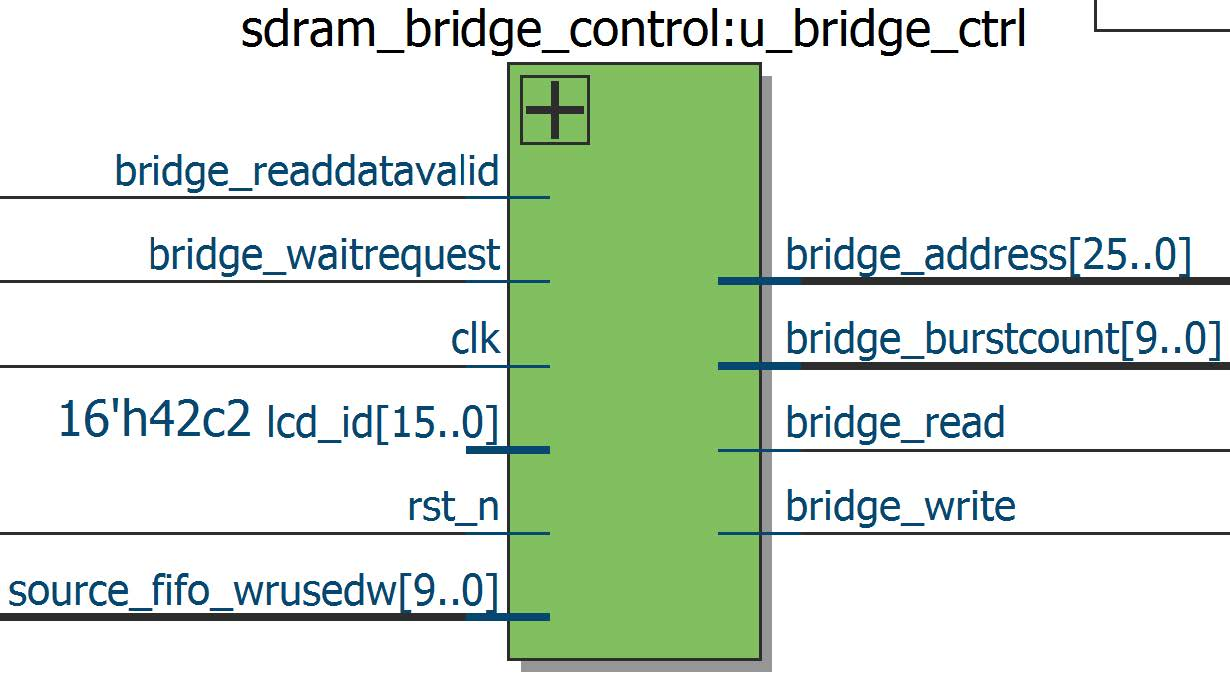
\includegraphics[width=0.5\textwidth]{SDRAM桥控制模块.jpg}
\end{figure}

\subsubsection{Qsys系统搭建}
在介绍完触摸驱动模块和SDRAM桥控制模块之后,接下来我们来介绍下Qsys系统环境的搭建,如下图所示:
  \begin{figure}[!htb]
	\centering
	\caption{Qsys系统的搭建}
	\label{Qsys系统的搭建}
	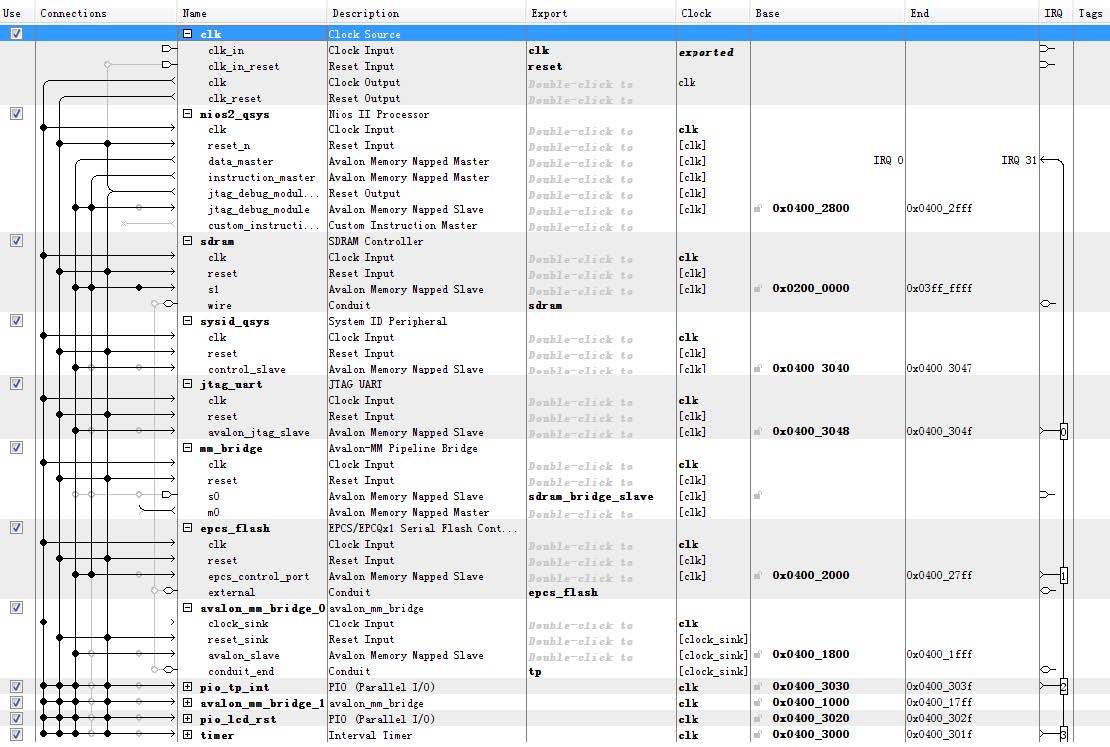
\includegraphics[width=0.9\textwidth]{Qsys系统的搭建.jpg}
\end{figure}
其中mm\_bridge用于以突发的方式从SDRAM中读出数据;avalon\_mm\_bridge\_0和avalon\_mm\_bridge\_1为自定义的IP核,分别用于获取触摸点坐标和配置显示界面的参数,pio\_tp\_int为PIO IP核,用于连接触摸屏模块输出的touch\_done(触摸完成信号),同时该PIO IP核设置了上升沿触发中断的功能,作为Nios II开始读取坐标点的标志;pio\_lcd\_rst同样为PIO IP核,只不过该IP核是作为Nios II的输出端口,用于控制LCD屏的复位;最后是添加的定时器IP核(timer),用于定时获取硬件中波形的频率和峰峰值。

Qsys系统模块接口如下图\ref{Qsys系统模块}所示:
  \begin{figure}[!htb]
	\centering
	\caption{Qsys系统模块}
	\label{Qsys系统模块}
	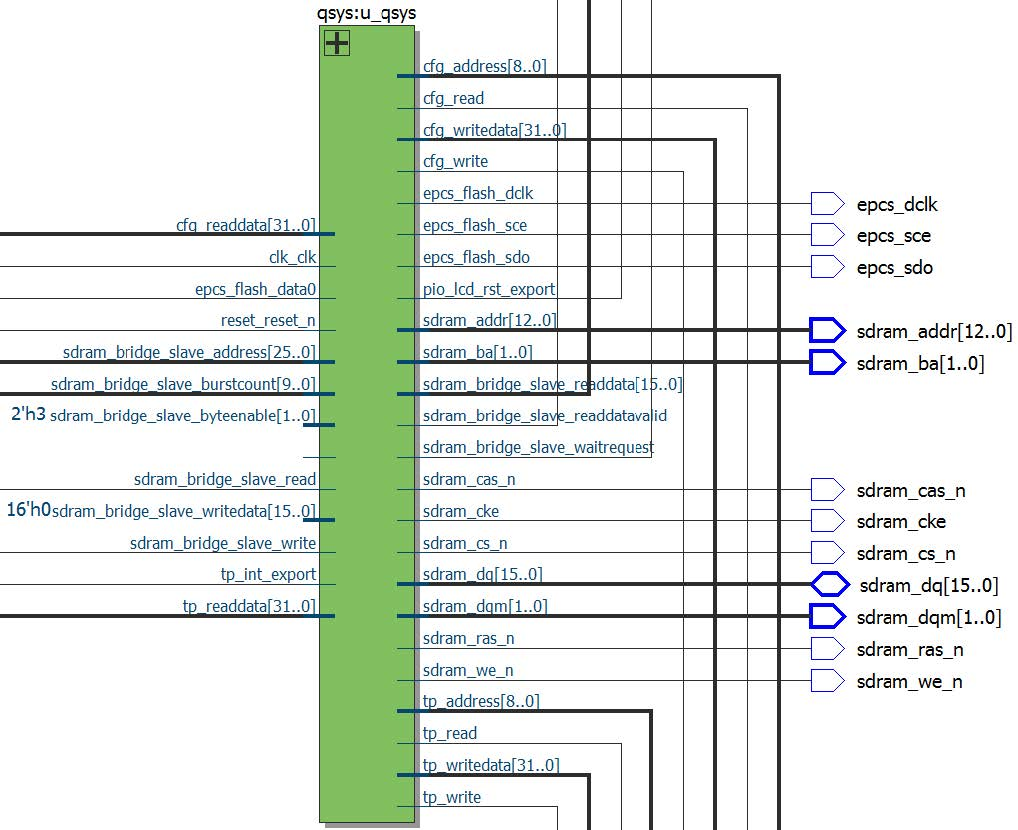
\includegraphics[width=0.5\textwidth]{Qsys系统模块.jpg}
\end{figure}

\subsubsection{Nios II软件设计}
在介绍完Qsys系统的搭建之后,最后我们再来介绍一下Nios II软件设计部分。

Nios II主要完成UI界面的绘制以及根据触摸屏输入的触摸点坐标来判断用户的按键操作。除此之外,Nios II还需要将从Avalon-MM端口中读取到的波形频率与峰峰值按照一定的格式,显示到界面上。

需要说明的是,由于波形的缩放、触发电平的位置显示等都是由硬件实现的,为了方便硬件实现这部分的功能,Nios II在通过Avalon-MM端口传输参数之前,要先对数据进行预处理,以降低硬件实现的复杂性。

最终,在RGB LCD屏上显示的界面如下图所示 \ref{用户界面}:
  \begin{figure}[!htb]
	\centering
	\caption{用户界面}
	\label{用户界面1}
	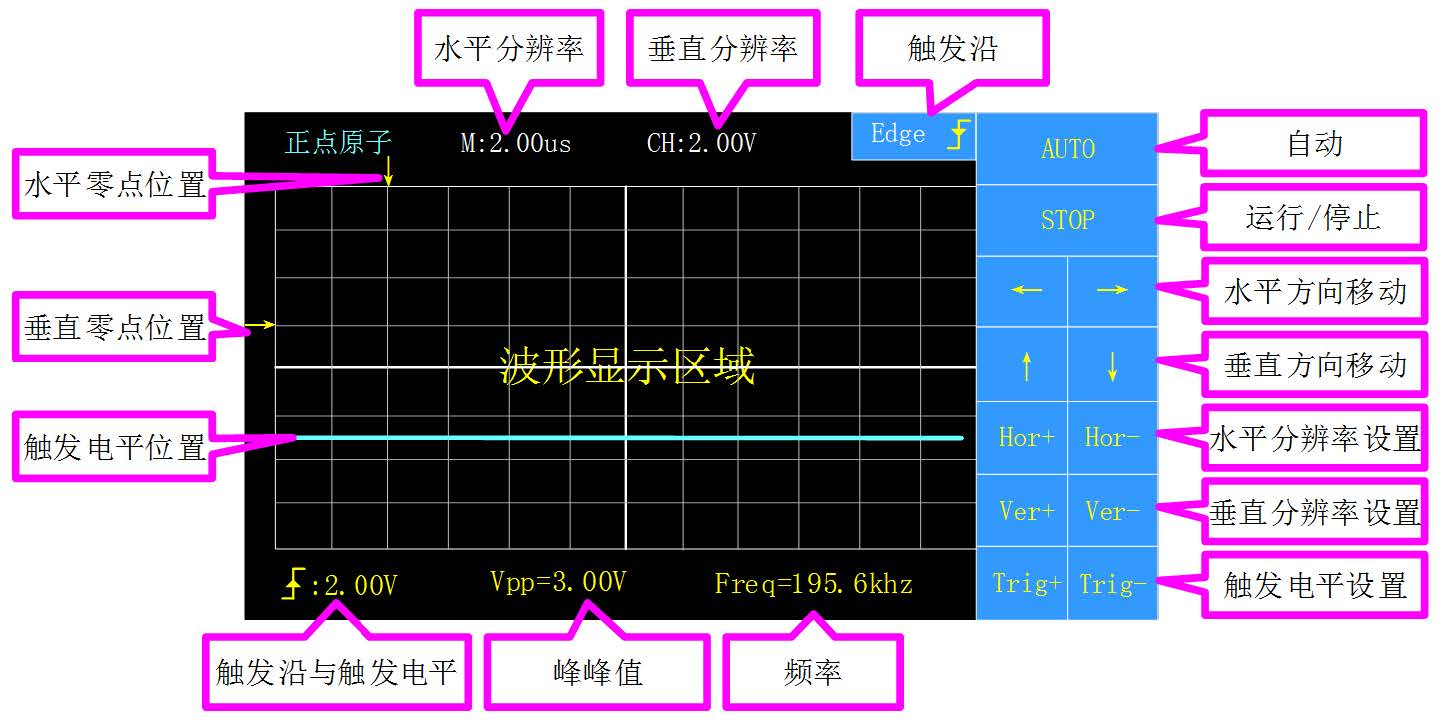
\includegraphics[width=0.9\textwidth]{用户界面.jpg}
\end{figure}

使用GUI\_DrawLine()函数实现画线的功能,GUI\_DrawRect()函数实现画矩形框的功能,GUI\_DispStringAt()函数实现显示字符串的功能。图中使用的汉字、字母、数字与箭头是由“uC-GUI-FontConvert”软件生成的字体,这里着重强调一下上升沿的字符和下降沿的字符是如何生成的。由于字符软件中并没有这个字符,所以我们对生成的字体文件做了修改,在字体软件中选中的字符如下图所示:
  \begin{figure}[!htb]
	\centering
	\caption{原始文件}
	\label{原始文件}
	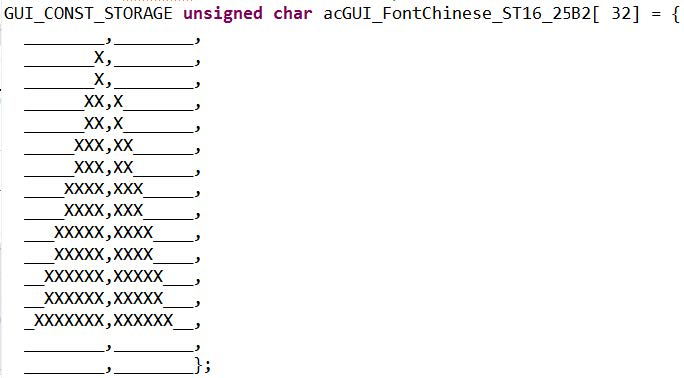
\includegraphics[width=0.9\textwidth]{原始文件.jpg}
\end{figure}
接下来对../uCGUI/Font/Chinese\_ST16.c文件中“▲”和“▼”对应的代码做修改,原始的文件和修改后的文件分别如图 26.4.9和图 26.4.10所示:
  \begin{figure}[!htb]
	\centering
	\caption{修改后的文件}
	\label{修改后的文件}
	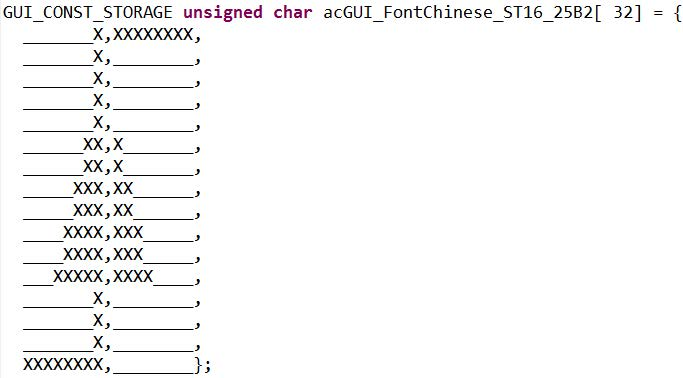
\includegraphics[width=0.9\textwidth]{修改后的文件.jpg}
\end{figure}
图中只展示了上升沿字符的修改方法,下降沿字符的修改方法也是一样的。代码修改完成后,接下来在字符显示函数中输入字符参数“▲”和“▼”时,在显示界面上看到的就会是上升沿和下降沿了。

接下来我们看下main函数的代码,了解下Nios II执行的过程。
\begin{lstlisting}
int main() 
{
	printf("Hello from NiosII!\n");
	IOWR_ALTERA_AVALON_PIO_DATA(PIO_LCD_RST_BASE,0); // LCD复位
	GUI_Init(); // uC/GUI初始化
	GUI_UC_SetEncodeUTF8(); // 设置字体
	GUI_SetFont(&GUI_FontChinese_ST16);
	init_tp_interrupt(); // 触摸中断初始化
	Timer_initial(); // 定时器中断初始化
	
	lcddev.width = 800; // 5'屏宽度
	lcddev.height = 480; // 5'屏高度
	IOWR_ALTERA_AVALON_PIO_DATA(PIO_LCD_RST_BASE,1); // LCD结束复位
	Draw_Display(); // 绘制显示界面
	SendCfgPara(); // 配置硬件参数
	
	while(1) {
		if(touch) // 检测到触摸中断
		{
			TouchPro(x_pos,y_pos); // 触摸处理
			touch = 0; // 清除触摸标志
		}
		
		// 定时器定时完成并且示波器正在运行
		if(timer_flag && dispdev.run_flag == 1) {
			GetDataDisp(); // 获取硬件数据
			timer_flag = 0; // 定时器标志清零
		}
	}
	
	return 0;
}
\end{lstlisting}
在软件代码中,我们添加了两个中断,第一个是触摸屏的PIO中断,作为开始获取触摸点坐标的标志;第二个是定时器的中断,作为开始获取波形频率和峰峰值的触发信号,这里之所以没有一直获取频率和峰峰值,是为了防止数据变化的速度太快,导致界面看不清频率和峰峰值的情况。在代码的第8行和第9行,实现的功能是分别对触摸屏的PIO中断和定时器中断进行初始化。

随后对LCD屏的分辨率进行设置,由于波形显示是横屏显示的,所以LCD屏的宽度和高度分别为800和480,然后结束LCD屏的复位。接下来就开始绘制显示界面了,由Draw\_Display()函数来完成,UI的初始界面以及数值的更新显示都是由这个函数来完成的,在绘制完界面后,需要将界面的初始化参数发送给硬件,即通过SendCfgPara()函数来实现。

接下来在while循环中判断触摸中断的标志(touch)和定时器完成标志(timer\_flag)是否为高电平。如果触摸中断标志为高电平,开始触摸点坐标的处理,代码中第86行输入的参数x\_pos和y\_pos,就是触摸点的x坐标和y坐标,TouchPro()函数根据触摸屏输入的触摸点坐标来判断用户的按键操作;当定时器完成标志为高电平时,开始获取波形频率和峰峰值,并显示在界面上。
\begin{lstlisting}
extern alt_u16 *ram;

int addr;

void LCD_DP(int x,int y,int color){
	addr = y * 800 + x;
	*(ram + addr) = color;
}
\end{lstlisting}

\section{系统调试}
	接下来我们把程序下载至征途开发板上,验证我们所完成的示波器的功能。
	首先把高速AD/DA模块和5寸RGB屏连接到征途开发板上,然后连接电源及JTAG接口。
	为了验证示波器的功能,我们在程序中利用高速AD/DA模块上的DA芯片输出了一个频率为
	195.3KHz的正弦波,因此还需要用两端都是公头的杜邦线将高速AD/DA模块的DA输出与AD输入
	连接起来。
	接下来打开电源,先Programmer中下载本次实验所生成的qsys\_gui\_oscp.sof文件,然后
	在Eclipse中下载qsys\_gui.elf文件。下载完成后,LCD上显示的界面如下所示:
	  \begin{figure}[!htb]
		\centering
		\caption{示波器效果图}
		\label{示波器效果图}
		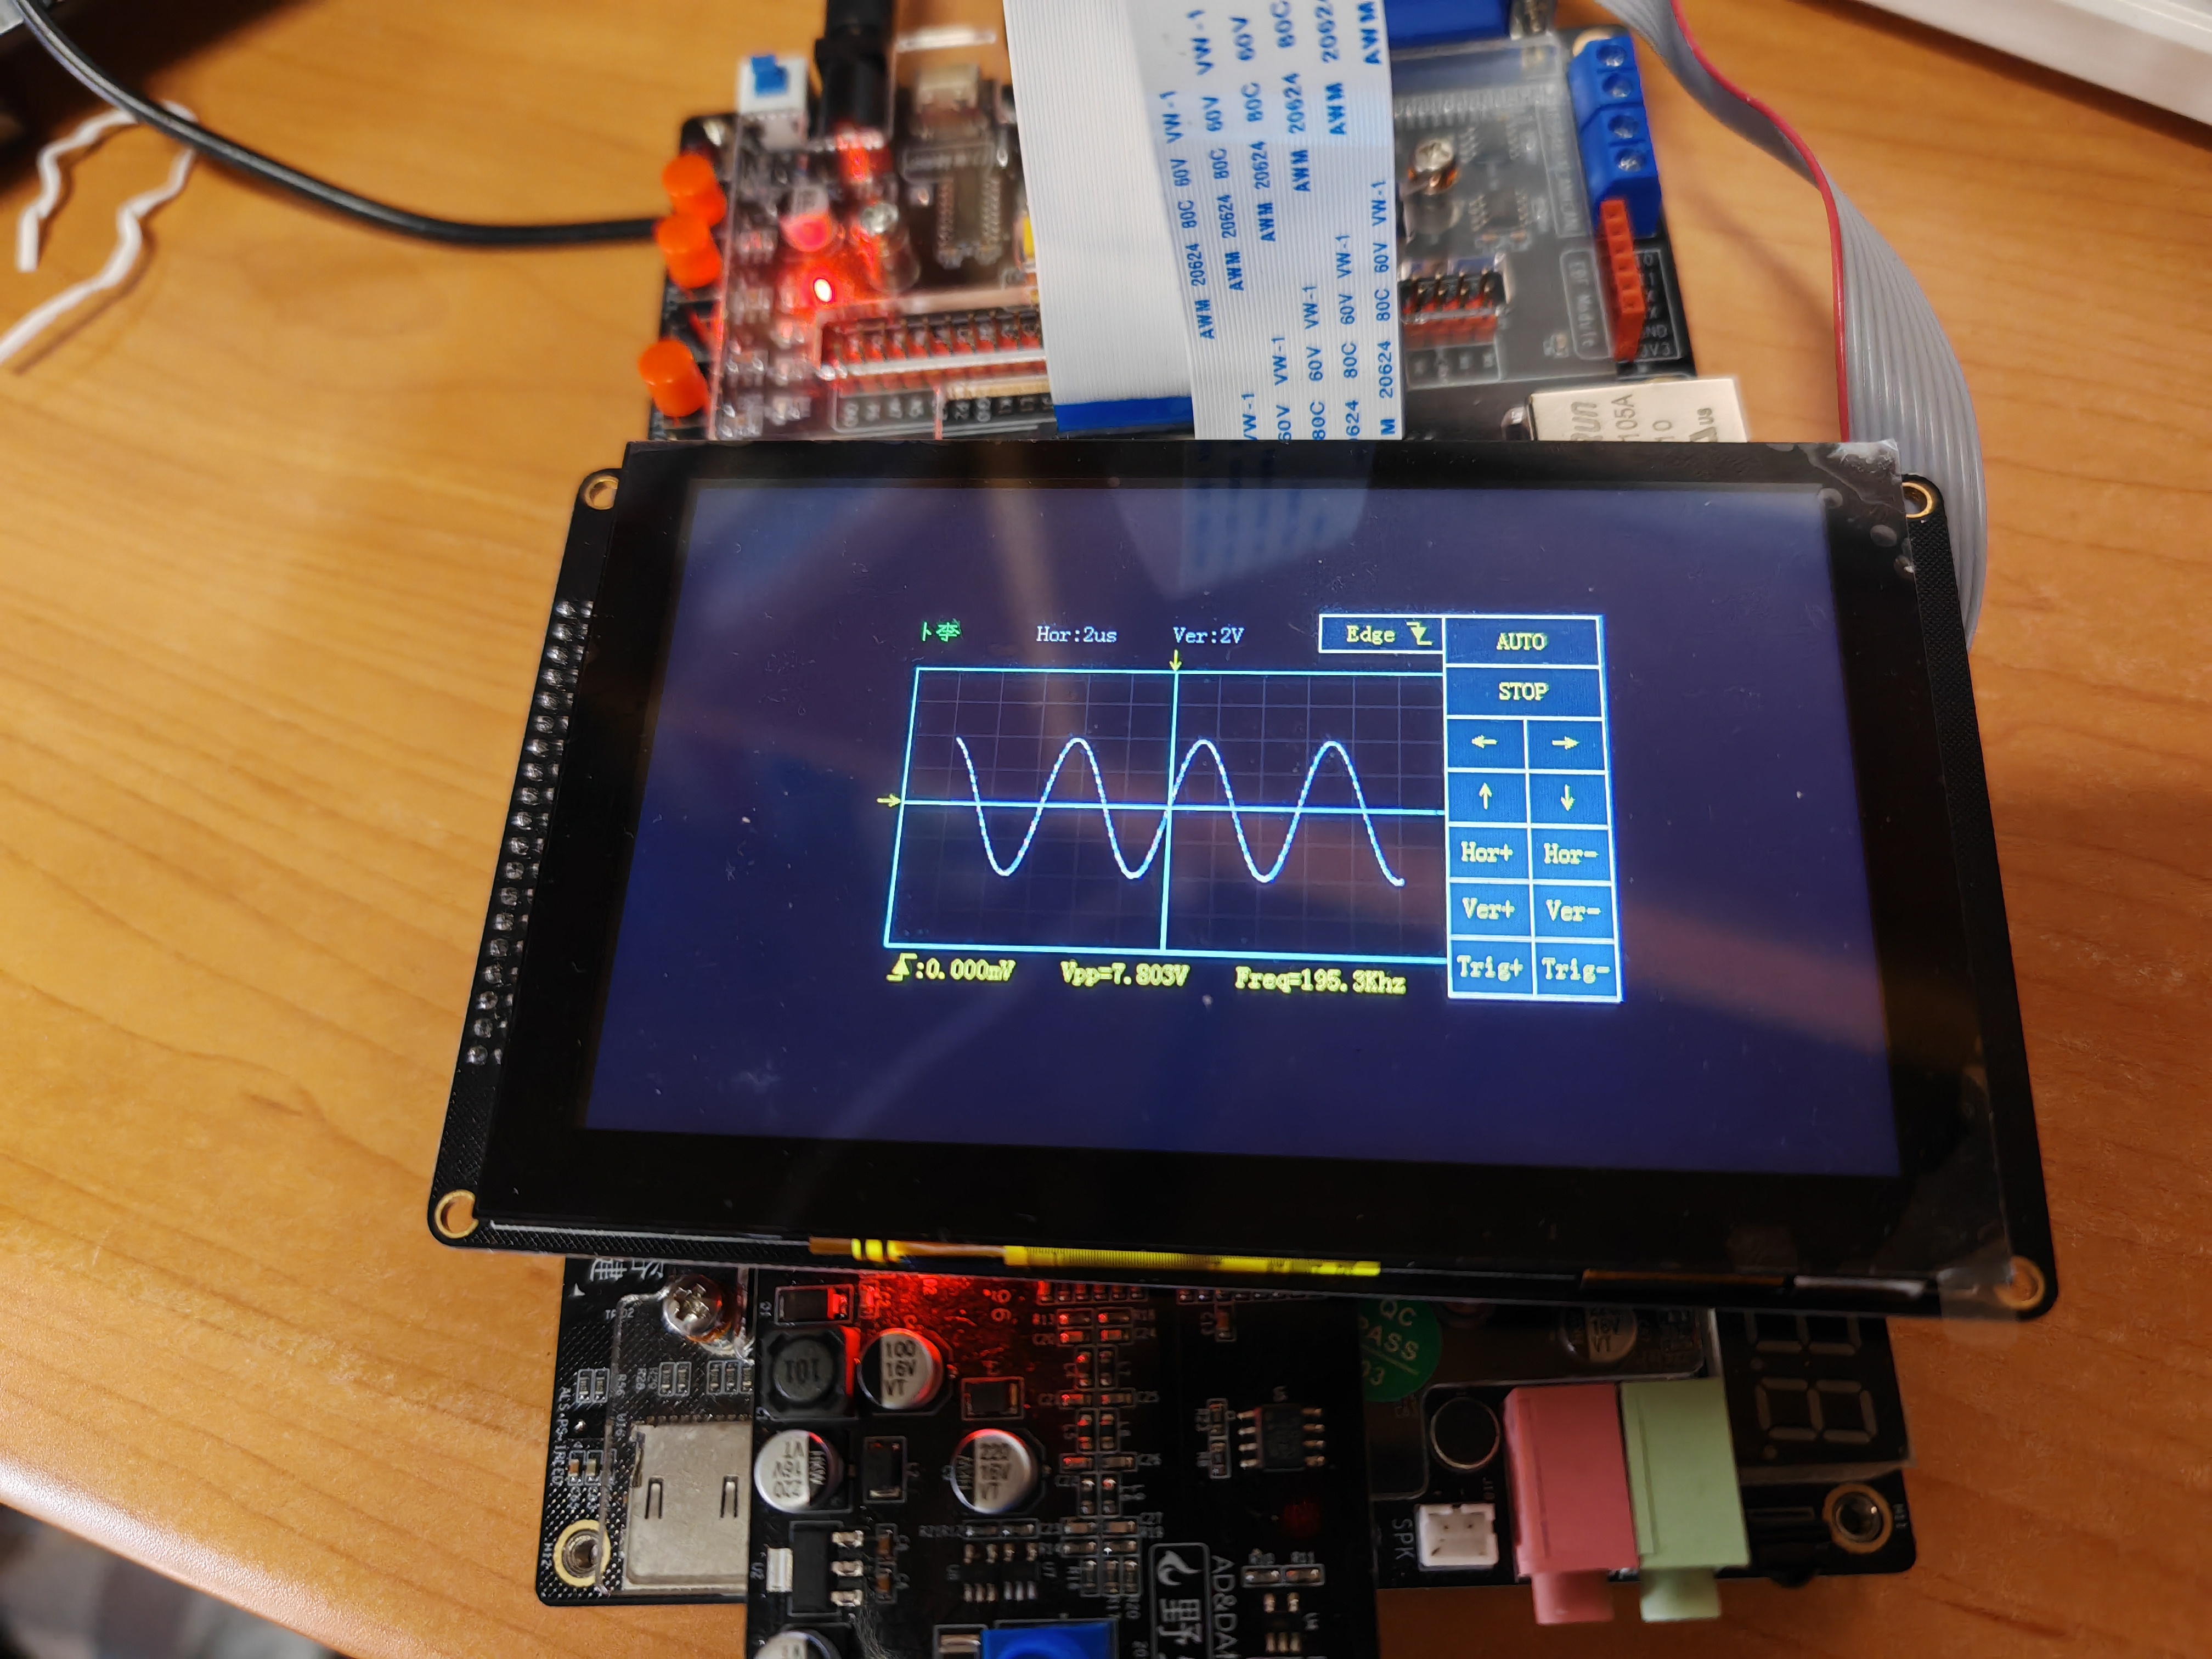
\includegraphics[width=0.9\textwidth]{示波器效果图.jpg}
	\end{figure}
\section{总结}
\subsection{项目总结}
	本项目成功设计并实现了一个基于野火FPGA征途Pro开发板和高速AD/DA模块的数字存储示波器。整个设计过程融合了硬件设计与软件编程,采用了Verilog HDL和C语言,实现了一个高效且功能齐全的示波器系统。
	
	硬件部分的设计关键在于将示波器的功能合理划分,并利用FPGA实现。这包括了波形的绘制和用户界面的绘制两个主要部分。波形绘制部分由FPGA硬件负责,采用Verilog HDL进行设计,以满足实时显示对图像刷新速率的高要求。而用户界面的绘制则更为复杂,需要软件的介入,因此在嵌入式处理器Nios II中使用C语言来实现。整个系统包含了多个关键的子模块,如测量模块用于信号的频率和峰峰值测量,抽取模块负责AD数据的抽样处理,存储模块用于数据存储和触发条件的判断,绘波形模块负责波形的具体绘制,以及Avalon-MM接口模块实现Nios II与各硬件模块的通信。
	
	在软件方面,主要任务是实现用户界面的绘制和用户交互逻辑。通过使用uC/GUI库在Nios II中实现了一个直观且易操作的用户界面,包括各种功能按键、波形参数显示等。此外,软件还负责处理触摸屏输入,实现用户对示波器功能的控制,如运行控制、触发控制、波形显示的水平和竖直方向控制等。Nios II还处理硬件模块传来的数据,并将测量结果如频率和峰峰值实时显示在界面上。
	
	整个系统的集成考虑了硬件与软件的协同工作。在硬件模块稳定运行的基础上,软件部分确保了用户界面的流畅交互和数据处理的准确性。通过实际的实验条件测试,系统展示了良好的稳定性和准确性,验证了设计的有效性。
	
	综上所述,该项目不仅展示了数字存储示波器在电子测量领域的应用,也体现了现代电子系统设计中硬件与软件相结合的重要性。通过这种跨学科的设计方法,可以实现复杂功能的电子设备,具有较高的实用价值和教育意义。

%本设计中,我们要利用正点原子高速 AD/DA 模块,在FPGA 开发板上实现一个数字存储示波器,利用 RGB LCD 屏显示波形和界面并测量信号的频率和峰峰值示波器界面基于 480*272 分辨率进行显示,在 4.3 寸 480*272 分辨率的 RGB LCD 屏上可以全屏显示,而在 5 寸 800*480分辨率下居中显示(四周填充黑边),而在设计的过程中,也碰到了很多问题,。
%  \begin{figure}[!htb]
%	\centering
%	\caption{elf文件下载失败的问题}
%	\label{elf文件下载失败的问题}
%	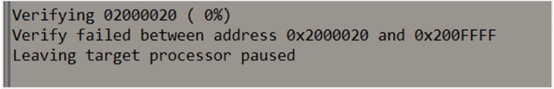
\includegraphics[width=0.9\textwidth]{李.png}
%\end{figure}
%比如:在设计完硬件后,在NIOSII中烧入elf文件时老是报错,经过反复调试,如图下所示,在QSYS系统中查看,发现验证失败地址所在为SDRAM地址,在重新分配基地址后发现并不是地址分配出错,而后又反复验证,发现是在硬件设计中引脚分配时 SDRAM的一个引脚分配出错,再更改后重新下载,烧入成功,所以在设计硬件时,尤其在分配引脚时要尤为小心,否则将严重推延设计进度。
%
%还有在驱动触摸屏时,发现触摸功能失效,发现示例驱动程序对应芯片为9147,而最新触摸屏芯片更改为1151,导致驱动不了芯片,读取坐标信息错误,在更改控制,状态,坐标寄存器地址后,触摸仍无反应,重新多次反复实验确认产品ID号,问题解决。


\subsection{不足与改进方向}


%本项目的不足如下:
%综上,尽管本项目取得了一定的成果,但在实际操作过程中仍发现了一些问题,未来改进方向包括:
%\begin{itemize}
%	\item 优化前端调理电路:降低输入噪声,提高信噪比。
%	\item 提升算法效率:通过改进或采用更先进的算法来降低处理延时和计算误差。
%	\item 完善人机交互界面:优化用户界面,提供更多自定义选项和高级功能,并能实际通过触摸屏进行波形的运行控制、触发控制以及水平和竖直方向控制。
%	\item 扩展接口兼容性: 增加与其他测量设备的接口兼容性,提高系统的集成能力。
%	\item 完善自动校准机制:引入自动校准功能减少人为误差和校准复杂性。
%\end{itemize}

虽然本项目在设计和实现上取得了显著成果,但仍存在一些不足之处,同时也提出了未来的改进和发展方向。
\begin{itemize}
	\item 性能限制: 目前系统的性能受限于所使用的FPGA开发板和AD/DA模块的性能。更高性能的硬件可能进一步提升示波器的测量准确度和数据处理能力。
	\item 功能扩展: 目前实现的功能相对基础,缺乏一些高级功能,如更复杂的信号分析、频谱分析等。
	\item 用户界面: 虽然用户界面已经实现了基本功能,但在易用性和美观性方面还有待提升。
	\item 实时性能: 在高频信号的处理和显示上,系统可能存在一定的延迟,影响了测量的实时性。
\end{itemize}
对此,我们有以下展望:

\begin{itemize}
	\item 硬件升级: 采用更高性能的FPGA和更先进的AD/DA模块,以提高整体处理能力和测量精度。
	\item 功能丰富化: 加入更多高级测量和分析功能,如数字滤波、频谱分析等,增强示波器的实用性。
	\item 用户界面优化: 改进用户界面设计,提高交互体验,例如增加触控反馈,优化布局和视觉设计,使操作更直观、便捷。
	\item 软件优化: 对软件进行进一步优化,提高数据处理和显示的实时性,减少延迟。
	\item 教育与研发应用: 将该项目作为教育和研发的平台,培养学生在硬件设计和软件编程方面的实践能力,同时为科研提供一个实验工具。
\end{itemize}

综上所述,本项目虽然在设计和实现上已经取得了一定成果,但仍有很大的发展空间。未来的改进和优化将使这个示波器系统更加强大和实用,更好地服务于教育和科研领域。


%\section{模板使用须知}
%
%\textcolor{red}{\bfseries 本模板自 2023 年 1 月 1 日开始,不再维护,不建议使用本系列模板!为了保证之前版本的用户仍然能查到说明文档,本说明文档仍然保留过去的信息。}
%
%\subsection{注意事项}
%\textbf{文献部分}:我们将 bibtex 的默认文献编译方式改为 biblatex,不过我们也提供了两个后端,\lstinline{bibend=biber} 和 \lstinline{bibend=bibtex}。特别需要注意的是从 0.10 开始,文献文件改为 \lstinline{reference.bib},与 ElegantBook 保持一致,而参考文献的引文样式等更多格式,请参考后文参考文献部分,更多样式可以参考 biblatex 文档。 
%
%\textbf{字体部分},我们将 newtxtext 宏包的支持方式改为了字体名称设定方式,设定英文字体为 TeX Gyre Terms/Heros,英文字体部分,根据编译方式选择不同字体。对于一般用户而言,不太需要关心这部分内容。
%
%另外,中文请务必使用 \hologo{XeLaTeX} 编译。
%
%\subsection{模板介绍}
%
%此模板基于 \LaTeX{} 的标准文类 article 设计,所以 article 文类的选项也能传递给本模板,比如 \lstinline{a4paper, 11pt} 等等。
%
%\begin{lstlisting}
%\documentclass[a4paper,11pt]{elegantpaper}
%\end{lstlisting}
%
%\textbf{注意}:Elegant\LaTeX{} 系列模板已经全部上传至 \href{https://www.overleaf.com/latex/templates/elegantpaper-template/yzghrqjhmmmr}{Overleaf} 上,用户可以在线使用。另外,为了方便国内用户,模板也已经传至\href{https://gitee.com/ElegantLaTeX/ElegantPaper}{码云}。
%
%
%\subsection{全局选项}
%此模板定义了一个语言选项 \lstinline{lang},可以选择英文模式 \lstinline{lang=en}(默认)或者中文模式 \lstinline{lang=cn}。当选择中文模式时,图表的标题引导词以及参考文献,定理引导词等信息会变成中文。你可以通过下面两种方式来选择语言模式:
%\begin{lstlisting}
%\documentclass[lang=cn]{elegantpaper} % or
%\documentclass[cn]{elegantpaper} 
%\end{lstlisting}
%
%\textbf{注意:} 英文模式下,由于没有添加中文宏包,无法输入中文。如果需要输入中文,可以通过在导言区引入中文宏包 \lstinline{ctex} 或者加入 \lstinline{xeCJK} 宏包后自行设置字体。 
%\begin{lstlisting}
%\usepackage[UTF8,scheme=plain]{ctex}
%\end{lstlisting}
%
%\subsection{数学字体选项}
%
%本模板定义了一个数学字体选项(\lstinline{math}),可选项有三个:
%\begin{enumerate}
%  \item \lstinline{math=cm}(默认),使用 \LaTeX{} 默认数学字体(推荐,无需声明);
%  \item \lstinline{math=newtx},使用 \lstinline{newtxmath} 设置数学字体(潜在问题比较多)。
%  \item \lstinline{math=mtpro2},使用 \lstinline{mtpro2} 宏包设置数学字体,要求用户已经成功安装此宏包。
%\end{enumerate}
%
%\subsection{中文字体选项}
%
%模板提供中文字体选项 \lstinline{chinesefont},可选项有
%\begin{enumerate}
%  \item \lstinline{ctexfont}:默认选项,使用 \lstinline{ctex} 宏包根据系统自行选择字体,可能存在字体缺失的问题,更多内容参考 \lstinline{ctex} 宏包\href{https://ctan.org/pkg/ctex}{官方文档}\footnote{可以使用命令提示符,输入 \lstinline{texdoc ctex} 调出本地 \lstinline{ctex} 宏包文档}。
%  \item \lstinline{founder}:方正字体选项(\textbf{需要安装方正字体}),后台调用 \lstinline{ctex} 宏包并且使用 \lstinline{fontset=none} 选项,然后设置字体为方正四款免费字体,方正字体下载注意事项见后文,用户只需要安装方正字体即可使用该选项。
%  \item \lstinline{nofont}:后台会调用 \lstinline{ctex} 宏包并且使用 \lstinline{fontset=none} 选项,不设定中文字体,用户可以自行设置中文字体,具体见后文。
%\end{enumerate}
%
%\subsubsection{方正字体选项}
%由于使用 \lstinline{ctex} 宏包默认调用系统已有的字体,部分系统字体缺失严重,因此,用户希望能够使用其它字体,我们推荐使用方正字体。方正的{\songti 方正书宋}、{\heiti 方正黑体}、{\kaishu 方正楷体}、{\fangsong 方正仿宋}四款字体均可免费试用,且可用于商业用途。用户可以自行从\href{http://www.foundertype.com/}{方正字体官网}下载此四款字体,在下载的时候请\textbf{务必}注意选择 GBK 字符集,也可以使用 \href{https://www.latexstudio.net/}{\LaTeX{} 工作室}提供的\href{https://pan.baidu.com/s/1BgbQM7LoinY7m8yeP25Y7Q}{方正字体,提取码为:njy9} 进行安装。安装时,{\kaishu Win 10 用户请右键选择为全部用户安装,否则会找不到字体。}
%
%\begin{figure}[!htb]
%\centering
%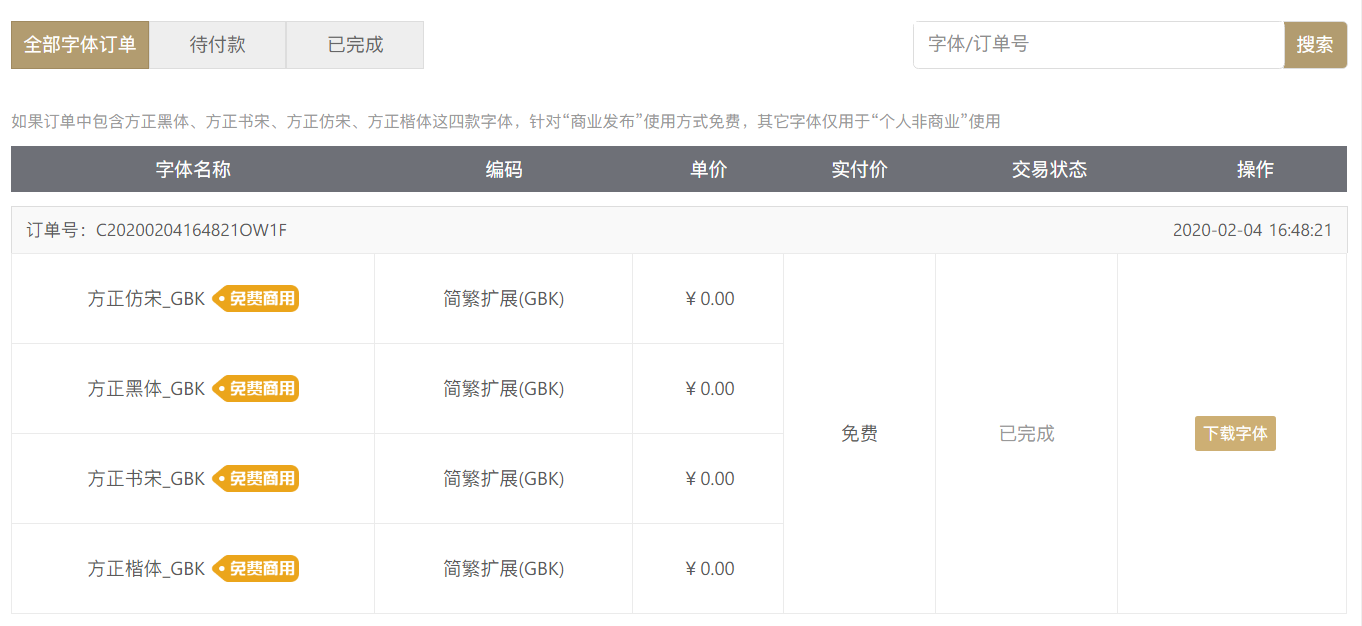
\includegraphics[width=0.9\textwidth]{founder.png}
%\end{figure}
%
%\subsubsection{其他中文字体}
%如果你想完全自定义字体\footnote{这里仍然以方正字体为例。},你可以选择 \lstinline{chinesefont=nofont},然后在导言区设置即可,可以参考下方代码:
%\begin{lstlisting}
%\setCJKmainfont[BoldFont={FZHei-B01},ItalicFont={FZKai-Z03}]{FZShuSong-Z01}
%\setCJKsansfont[BoldFont={FZHei-B01}]{FZKai-Z03}
%\setCJKmonofont[BoldFont={FZHei-B01}]{FZFangSong-Z02}
%\setCJKfamilyfont{zhsong}{FZShuSong-Z01}
%\setCJKfamilyfont{zhhei}{FZHei-B01}
%\setCJKfamilyfont{zhkai}[BoldFont={FZHei-B01}]{FZKai-Z03}
%\setCJKfamilyfont{zhfs}[BoldFont={FZHei-B01}]{FZFangSong-Z02}
%\newcommand*{\songti}{\CJKfamily{zhsong}}
%\newcommand*{\heiti}{\CJKfamily{zhhei}}
%\newcommand*{\kaishu}{\CJKfamily{zhkai}}
%\newcommand*{\fangsong}{\CJKfamily{zhfs}}
%\end{lstlisting}
%
%
%
%\subsection{自定义命令}
%此模板并没有修改任何默认的 \LaTeX{} 命令或者环境\footnote{目的是保证代码的可复用性,请用户关注内容,不要太在意格式,这才是本工作论文模板的意义。}。另外,本模板可以使用的 4 个额外命令:
%\begin{enumerate}
%  \item \lstinline{\email}:创建邮箱地址的链接,比如 \email{xxx@outlook.com};
%  \item \lstinline{\figref}:用法和 \lstinline{\ref} 类似,但是会在插图的标题前添加 <\textbf{图 n}> ;
%  \item \lstinline{\tabref}:用法和 \lstinline{\ref} 类似,但是会在表格的标题前添加 <\textbf{表 n}>;
%  \item \lstinline{\keywords}:为摘要环境添加关键词。
%\end{enumerate}
%
%\subsection{参考文献}
%
%文献部分,本模板调用了 biblatex 宏包,并提供了 biber(默认) 和 bibtex 两个后端选项,可以使用 \lstinline{bibend} 进行修改:
%
%\begin{lstlisting}
%  \documentclass[bibtex]{elegantpaper}
%  \documentclass[bibend=bibtex]{elegantpaper}
%\end{lstlisting}
%
%关于文献条目(bib item),你可以在谷歌学术,Mendeley,Endnote 中取,然后把它们添加到 \lstinline{reference.bib} 中。在文中引用的时候,引用它们的键值(bib key)即可。
%
%为了方便文献样式修改,模板引入了 \lstinline{bibstyle} 和 \lstinline{citestyle} 选项,默认均为数字格式(numeric),参考文献示例:\cite{cn1,en2,en3} 使用了中国一个大型的 P2P 平台(人人贷)的数据来检验男性投资者和女性投资者在投资表现上是否有显著差异。
%
%如果需要设置为国标 GB7714-2015,需要使用:
%\begin{lstlisting}
%  \documentclass[citestyle=gb7714-2015, bibstyle=gb7714-2015]{elegantpaper} 
%\end{lstlisting}
%
%如果需要添加排序方式,可以在导言区加入
%\begin{lstlisting}
%  \ExecuteBibliographyOptions{sorting=ynt}
%\end{lstlisting}
%
%启用国标之后,可以加入 \lstinline{sorting=gb7714-2015}。
%
%
%\section{使用 newtx 系列字体}
%
%如果需要使用原先版本的 \lstinline{newtx} 系列字体,可以通过显示声明数学字体:
%
%\begin{lstlisting}
%\documentclass[math=newtx]{elegantpaper}
%\end{lstlisting}
%
%\subsection{连字符}
%
%如果使用 \lstinline{newtx} 系列字体宏包,需要注意下连字符的问题。
%\begin{equation}
%  \int_{R^q} f(x,y) dy.\emph{of\kern0pt f}
%\end{equation}
%
%\begin{lstlisting}
%\begin{equation}
%  \int_{R^q} f(x,y) dy.\emph{of \kern0pt f}
%\end{equation}
%\end{lstlisting}
%
%\subsection{宏包冲突}
%
%有用户反馈模板在使用 \lstinline{yhmath} 以及 \lstinline{esvect} 等宏包时会报错:
%\begin{lstlisting}
%LaTeX Error:
%   Too many symbol fonts declared.
%\end{lstlisting}
%
%原因是在使用 \lstinline{newtxmath} 宏包时,重新定义了数学字体用于大型操作符,达到了 {\heiti 最多 16 个数学字体} 的上限,在调用其他宏包的时候,无法新增数学字体。为了减少调用非常用宏包,在此给出如何调用 \lstinline{yhmath} 以及 \lstinline{esvect} 宏包的方法。
%
%请在 \lstinline{elegantpaper.cls} 内搜索 \lstinline{yhmath} 或者 \lstinline{esvect},将你所需要的宏包加载语句\textit{取消注释}即可。
%
%
%\section{常见问题 FAQ}
%
%\begin{enumerate}[label=\arabic*).]
%  \item \textit{如何删除版本信息?}\\
%    导言区不写 \lstinline|\version{x.xx}| 即可。
%  \item \textit{如何删除日期?}\\
%    需要注意的是,与版本 \lstinline{\version} 不同的是,导言区不写或注释 \lstinline{\date} 的话,仍然会打印出当日日期,原因是 \lstinline{\date} 有默认参数。如果不需要日期的话,日期可以留空即可,也即 \lstinline|\date{}|。
%  \item \textit{如何获得中文日期?}\\
%    为了获得中文日期,必须在中文模式下\footnote{英文模式下,由于未加载中文宏包,无法输入中文。},使用 \lstinline|\date{\zhdate{2019/10/11}}|,如果需要当天的汉化日期,可以使用 \lstinline|\date{\zhtoday}|,这两个命令都来源于 \href{https://ctan.org/pkg/zhnumber}{\lstinline{zhnumber}} 宏包。
%  \item \textit{如何添加多个作者?}\\
%    在 \lstinline{\author} 里面使用 \lstinline{\and},作者单位可以用 \lstinline{\\} 换行。
%    \begin{lstlisting}
%    \author{author 1\\ org. 1 \and author 2 \\ org. 2 }
%    \end{lstlisting}
%  \item \textit{如何添加中英文摘要?}\\
%    请参考 \href{https://github.com/ElegantLaTeX/ElegantPaper/issues/5}{GitHub::ElegantPaper/issues/5}
%\end{enumerate}
%
%
%\section{致谢}

%特别感谢 \href{https://github.com/sikouhjw}{sikouhjw} 和 \href{https://github.com/syvshc}{syvshc}  长期以来对于 Github 上 issue 的快速回应,以及各个社区论坛对于 ElegantLaTeX 相关问题的回复。特别感谢 ChinaTeX 以及 \href{http://www.latexstudio.net/}{LaTeX 工作室} 对于本系列模板的大力宣传与推广。
%
%如果你喜欢我们的模板,你可以在 Github 上收藏我们的模板。

\nocite{*}
\printbibliography[heading=bibintoc, title=\ebibname]

\appendix
%\appendixpage
\addappheadtotoc

\end{document}
